\documentclass[12pt,a4paper]{article}

\usepackage[T2A]{fontenc}
\usepackage[utf8]{inputenc}
\usepackage[russian]{babel}
\usepackage{amsmath,amssymb,amsfonts}
\usepackage{geometry}
\usepackage{graphicx}
\usepackage{subcaption}
\usepackage{booktabs}
\usepackage{float}
\usepackage{hyperref}
\usepackage[nameinlink,noabbrev]{cleveref}

\geometry{left=25mm,right=20mm,top=22mm,bottom=22mm}
\graphicspath{{./}{images/}}

\newcommand{\dd}{\,d}
\newcommand{\Reynolds}{\operatorname{Re}}
\newcommand{\Laplace}{\Delta}
\newcommand{\norm}[1]{\left\lVert #1 \right\rVert}
\newcommand{\inner}[2]{\left\langle #1,#2 \right\rangle}
\crefname{equation}{формуле}{формулах}
\crefname{figure}{рисунке}{рисунках}
\crefname{section}{разделе}{разделах}
\Crefname{equation}{Формула}{Формулы}
\Crefname{figure}{Рисунок}{Рисунки}
\Crefname{section}{Раздел}{Разделы}

\begin{document}

\begin{titlepage}
    \centering

    {\large Московский государственный университет имени М.\,В.~Ломоносова\par}
    \vspace{0.5em}
    {\large Механико-математический факультет\par}

    \vfill

    {\Large\bfseries Курсовая работа\par}
    \vspace{1.2em}
    {\LARGE\bfseries Численное моделирование двумерных течений\\[0.25em]
    в переменных функция тока--завихренность\\[0.25em]
    и подавление неустойчивых мод\par}

    \vfill

    \begin{flushright}
        \begin{minipage}{0.45\textwidth}
            Студент 4 курса\\
            механико-математического факультета

            \vspace{1.5em}
            Научный руководитель
        \end{minipage}
    \end{flushright}

    \vfill

    {\large Москва, 2026}
\end{titlepage}

\clearpage
\tableofcontents
\clearpage

\section{Введение}

Двумерные модели вязкой несжимаемой жидкости занимают особое место в вычислительной гидродинамике.
С одной стороны, они существенно проще трёхмерных уравнений Навье--Стокса и позволяют подробно изучать структуру численного метода.
С другой стороны, уже в двумерном случае возникают пограничные слои, вторичные вихри, потеря устойчивости стационарного режима и чувствительность решения к сетке.
Поэтому такие задачи хорошо подходят для курсовой работы по численным методам: в них видны и физика, и математика, и практические ограничения вычислений.

Основные переменные в этой работе --- функция тока \(\psi\) и завихренность \(\omega\).
В такой записи двумерное несжимаемое течение описывается эллиптическим уравнением для \(\psi\) и эволюционным уравнением для \(\omega\).
Именно эта форма используется во всех разностных алгоритмах ниже.

Первая задача --- течение в квадратной каверне с движущейся верхней стенкой, подробно исследованное в работе Erturk, Corke и G\"ok\c{c}\"ol~\cite{erturk2005}.
В проекте эта задача соответствует реализации с обычной центрально-разностной аппроксимацией конвективного члена.

Вторая часть --- вычислительный эксперимент с четырёхвихревой структурой в прямоугольной ячейке, мотивированный работой А.\,А.~Корнева~\cite{kornev2018}.
Сразу используется постановка в переменных \((\psi,\omega)\), поскольку именно в этих переменных написан разностный алгоритм.
Особый интерес представляет не только получение четырёх вихрей, но и стабилизация динамики около неустойчивого стационарного состояния.
Для этого строится линеаризованный оператор, находятся собственные значения с положительной действительной частью, а затем из решения вычитается проекция на соответствующие неустойчивые моды.

\section{Постановка задачи о каверне}

\subsection{Физическая постановка}

Рассматривается квадратная область
\begin{equation}
    \Omega=(0,1)\times(0,1),
    \label{eq:cavity-domain}
\end{equation}
заполненная вязкой несжимаемой жидкостью.
Верхняя стенка движется горизонтально с постоянной безразмерной скоростью \(U=1\), а левая, правая и нижняя стенки неподвижны.
Именно движение крышки возбуждает течение: возле верхней границы возникает сдвиговый слой, который передаёт импульс внутрь области и формирует главный вихрь.
При увеличении числа Рейнольдса пограничные слои становятся тоньше, главный вихрь смещается, а в углах появляются малые вторичные и третичные вихри.

В переменных \((\psi,\omega)\) движение крышки не задаётся как отдельное уравнение внутри области.
Оно входит через граничное условие для завихренности: на верхней стенке в формуле Тома появляется тангенциальная скорость \(U=1\), а на остальных стенках соответствующая скорость равна нулю.
Единственный безразмерный параметр задачи --- число Рейнольдса, которое в дальнейшем записывается через безразмерный коэффициент вязкости \(\nu\):
\begin{equation}
    \Reynolds=\frac{1}{\nu}.
    \label{eq:reynolds}
\end{equation}
В вычислительной реализации для этого теста использовалась сетка \(101\times101\) и значение \(\Reynolds=1/\nu=5000\), то есть \(\nu=1/5000\).

\subsection{Уравнения в переменных \texorpdfstring{\((\psi,\omega)\)}{psi, omega}}

В безразмерной постановке функция тока и завихренность связаны уравнением Пуассона
\begin{equation}
    \Laplace\psi+\omega=0.
    \label{eq:poisson-cavity}
\end{equation}
Уравнение для завихренности записывается в виде
\begin{equation}
    \frac{\partial\omega}{\partial t}
    =
    \nu\Laplace\omega
    +
    \psi_x\omega_y-\psi_y\omega_x.
    \label{eq:cavity-vorticity-evolution}
\end{equation}
Стационарная форма, используемая для контроля сходимости, имеет вид
\begin{equation}
    \nu\Laplace\omega+\psi_x\omega_y-\psi_y\omega_x=0.
    \label{eq:cavity-steady-vorticity}
\end{equation}
В работе~\cite{erturk2005} эта же система записана в форме \(\nu\Laplace\omega=\psi_y\omega_x-\psi_x\omega_y\), что эквивалентно \eqref{eq:cavity-steady-vorticity} при \(\Reynolds=1/\nu\).

\subsection{Граничные условия для \texorpdfstring{\(\psi\)}{psi} и \texorpdfstring{\(\omega\)}{omega}}

На твёрдой непроницаемой стенке нормальная скорость равна нулю.
Для функции тока это означает, что \(\psi\) постоянна вдоль каждой связной компоненты границы.
В замкнутой каверне расход через границу отсутствует, поэтому эту постоянную можно выбрать равной нулю:
\begin{equation}
    \psi\big|_{\partial\Omega}=0.
    \label{eq:cavity-psi-bc}
\end{equation}

Завихренность на стенке не задаётся независимо.
Она должна быть согласована с условием прилипания скорости.
В реализации используется формула Тома, которая выражает граничное значение \(\omega\) через ближайшее внутреннее значение функции тока и заданную тангенциальную скорость стенки.
Для равномерной сетки с шагами \(h_x,h_y\) получаем
\begin{equation}
\begin{aligned}
    \omega_{i,0}
    &=-\frac{2\psi_{i,1}}{h_y^2},\\
    \omega_{i,N_y}
    &=-\frac{2\psi_{i,N_y-1}}{h_y^2}-\frac{2U}{h_y},\\
    \omega_{0,j}
    &=-\frac{2\psi_{1,j}}{h_x^2},\\
    \omega_{N_x,j}
    &=-\frac{2\psi_{N_x-1,j}}{h_x^2}.
\end{aligned}
\label{eq:thom-cavity}
\end{equation}
Добавка \(-2U/h_y\) на верхней границе отвечает движущейся крышке.
На неподвижных стенках соответствующая тангенциальная скорость равна нулю, и остаётся только член с \(\psi\).
Локально формула Тома имеет первый порядок у стенки, однако при центральной аппроксимации во внутренних узлах глобальное решение сохраняет второй порядок по пространству для гладких решений; это также отмечается в~\cite{erturk2005}.

\section{Разностная схема для задачи о каверне}

\subsection{Сетка и сеточные функции}

Введём равномерную сетку
\begin{equation}
    x_i=ih_x,\quad i=0,\ldots,N_x,
    \qquad
    y_j=jh_y,\quad j=0,\ldots,N_y,
    \label{eq:grid}
\end{equation}
где \(h_x=1/N_x\), \(h_y=1/N_y\).
Сеточные значения на псевдовременном слое \(t^n=n\tau\) обозначаются
\[
    \psi_{i,j}^n\approx\psi(x_i,y_j,t^n),
    \qquad
    \omega_{i,j}^n\approx\omega(x_i,y_j,t^n).
\]
Все основные поля хранятся в узлах одной и той же сетки.
Такой выбор проще, чем разнесённые сетки, и хорошо согласуется с формулировкой через \(\psi\) и \(\omega\): все разностные операторы действуют на узловые сеточные функции с одним и тем же шаблоном.

\subsection{Разностные операторы}

Для первой производной используются центральные разности
\begin{equation}
    (D_x f)_{i,j}=\frac{f_{i+1,j}-f_{i-1,j}}{2h_x},
    \qquad
    (D_y f)_{i,j}=\frac{f_{i,j+1}-f_{i,j-1}}{2h_y}.
    \label{eq:central-first}
\end{equation}
Дискретный лапласиан имеет вид
\begin{equation}
    (\Laplace_h f)_{i,j}
    =
    \frac{f_{i+1,j}-2f_{i,j}+f_{i-1,j}}{h_x^2}
    +
    \frac{f_{i,j+1}-2f_{i,j}+f_{i,j-1}}{h_y^2}.
    \label{eq:discrete-laplacian}
\end{equation}
Нелинейный конвективный член в варианте для каверны аппроксимируется обычными центральными разностями:
\begin{equation}
    N_h^{(c)}(\psi,\omega)_{i,j}
    =
    (D_x\psi)_{i,j}(D_y\omega)_{i,j}
    -
    (D_y\psi)_{i,j}(D_x\omega)_{i,j}.
    \label{eq:central-nonlinearity}
\end{equation}
Именно \eqref{eq:central-nonlinearity} является реализованной формулой для этой части.
Преимущество такой аппроксимации --- простота и прозрачная связь с дифференциальным оператором.
Для стационарного теста о каверне это естественный выбор: основной вопрос здесь --- согласованное решение Пуассона, завихренности и граничных условий.

\subsection{Псевдовременная факторизация}

В работе~\cite{erturk2005} стационарная система решается как предел псевдовременной эволюции.
Для уравнения Пуассона вводится уравнение
\begin{equation}
    \psi_t=\Laplace\psi+\omega,
    \label{eq:pseudo-psi}
\end{equation}
а для завихренности используется \eqref{eq:cavity-vorticity-evolution}.
Неявный шаг Эйлера для \eqref{eq:pseudo-psi} дал бы большую разреженную систему
\[
    (I-\tau\Laplace_h)\psi^{n+1}=\psi^n+\tau\omega^n.
\]
В реализации используется приближённая факторизация по направлениям:
\begin{equation}
    (I-\tau D_{xx})(I-\tau D_{yy})\psi^{n+1}
    =
    \psi^n+\tau\omega^n
    +
    O(\tau^2).
    \label{eq:psi-factorized}
\end{equation}
Последний член в правой части не является искусственной вязкостью.
Он компенсирует \(O(\tau^2)\)-член, возникающий при факторизации, чтобы в стационарном пределе сохранялось правильное уравнение \(\Laplace_h\psi+\omega=0\).

Для завихренности применяется аналогичная факторизация с неявной диффузией и конвективными коэффициентами, вычисленными по текущей функции тока:
\begin{equation}
\begin{aligned}
    &\left(I-\tau\nu D_{xx}
        +\tau(D_y\psi^n)D_x\right)
     \left(I-\tau\nu D_{yy}
        -\tau(D_x\psi^n)D_y\right)\omega^{n+1}
    \\
    &\qquad =
    \omega^n+O(\tau^2),
\end{aligned}
\label{eq:omega-factorized}
\end{equation}
где \(O(\tau^2)\)-поправки снова вводятся для компенсации ошибки факторизации в стационарном пределе.
После разложения по направлениям каждая подзадача сводится к трёхдиагональной системе, решаемой методом прогонки.
Таким образом, вместо одной большой двумерной системы на каждом шаге решаются наборы одномерных задач по строкам и столбцам.

По времени схема является схемой первого порядка, поскольку псевдовременные производные аппроксимируются неявным Эйлером.
По пространству во внутренних узлах используются центральные разности второго порядка.
Следовательно, на гладких решениях ожидается второй порядок по пространству и первый порядок по псевдовремени.
Для стационарного решения главное значение имеет пространственная точность и величина стационарной невязки.

\section{Реализация и хранение данных для задачи о каверне}

В реализации хранятся четыре основные сеточные функции:
\[
    \psi_{i,j},\qquad \omega_{i,j},\qquad u_{i,j},\qquad v_{i,j}.
\]
Дополнительно используются вспомогательные массивы \(f\) и \(g\), возникающие при факторизации уравнений для \(\psi\) и \(\omega\).
Массив \(f\) соответствует промежуточному решению в \eqref{eq:psi-factorized}, а \(g\) --- промежуточному решению в \eqref{eq:omega-factorized}.
После обновления \(\psi\) применяется формула Тома \eqref{eq:thom-cavity}, затем обновляется \(\omega\), после чего вычисляются компоненты скорости для сохранения снимков и построения линий тока.

Один псевдовременной шаг можно описать так:
\begin{enumerate}
    \item построить правую часть для уравнения функции тока;
    \item решить трёхдиагональные системы по \(x\), затем по \(y\), получив \(\psi^{n+1}\);
    \item восстановить граничные значения завихренности по формуле Тома;
    \item построить правую часть для уравнения завихренности;
    \item решить факторизованную задачу для \(\omega^{n+1}\);
    \item вычислить стационарные невязки уравнений \eqref{eq:poisson-cavity} и \eqref{eq:cavity-steady-vorticity}.
\end{enumerate}
Такая структура хранения естественна для сеточного метода: все операторы локальны, а прогонка работает с одномерными срезами двумерных массивов.

\section{Результаты вычислений для задачи о каверне}

Для проверки реализации был выполнен расчёт классической задачи о каверне на сетке \(601\times601\), то есть на той же сетке, на которой в работе~\cite{erturk2005} приведены финальные контуры для больших чисел Рейнольдса.
Рассматривались три режима:
\[
    \Reynolds=1000,\qquad
    \Reynolds=5000,\qquad
    \Reynolds=10000.
\]
Шаг по псевдовремени во всех расчётах равен \(\tau=10^{-4}\), верхняя стенка движется со скоростью \(u=1\), остальные стенки неподвижны.
Правая часть отсутствует: течение создаётся только граничным условием на крышке.
Для каждого числа Рейнольдса ниже приведены линии тока.

\begin{figure}[H]
    \centering
    \begin{subfigure}{0.32\textwidth}
        \centering
        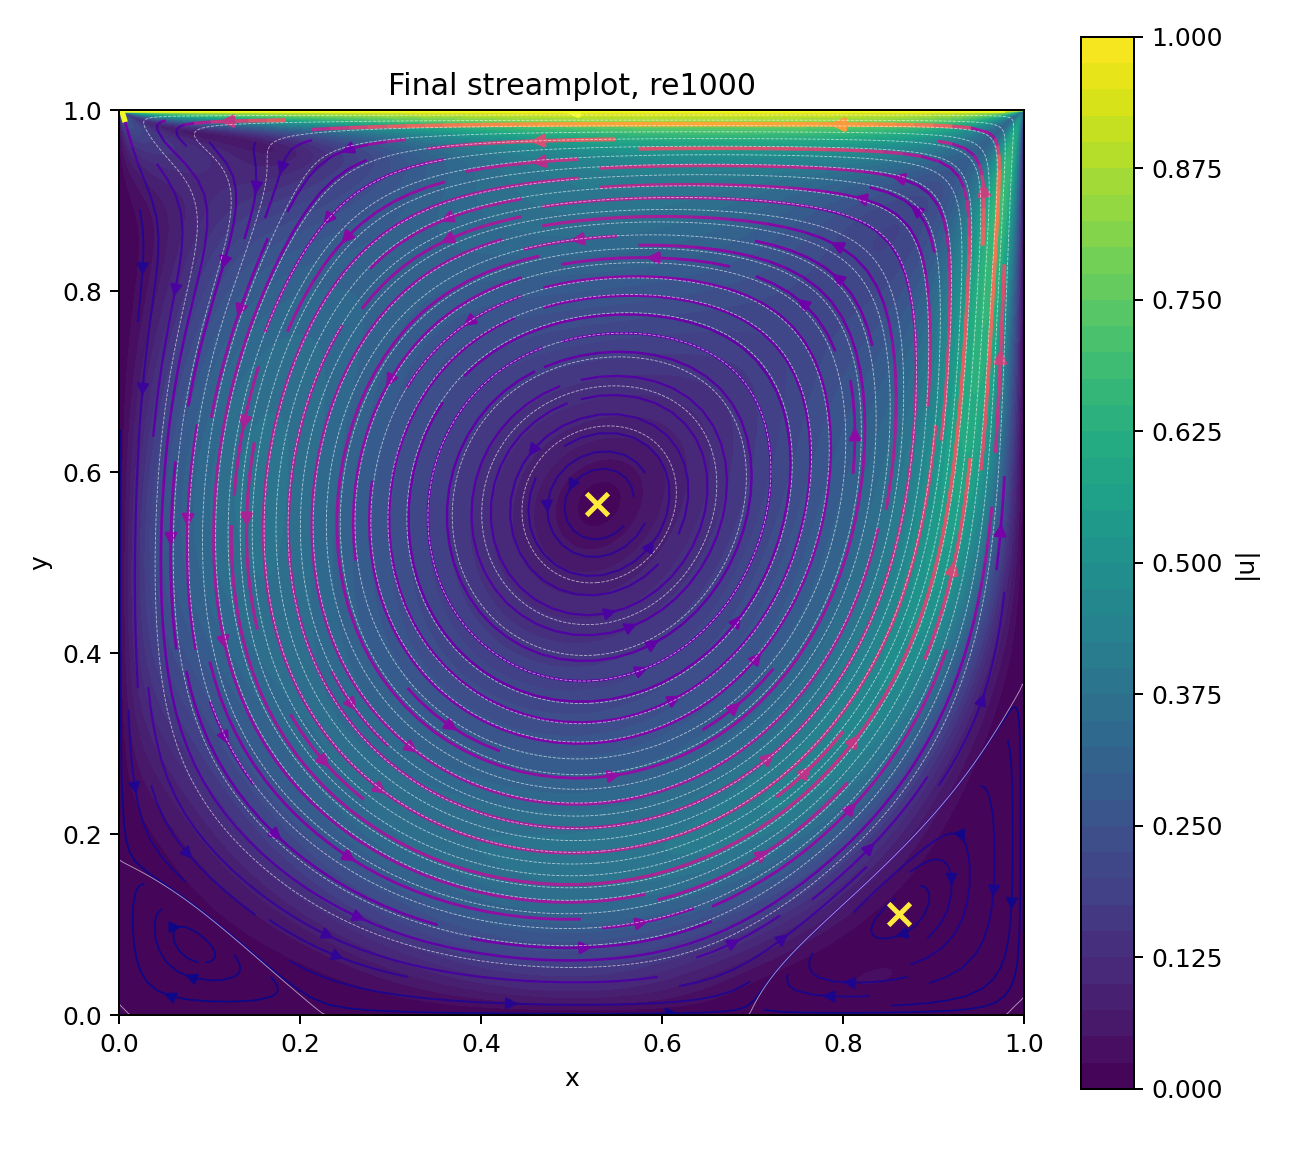
\includegraphics[width=\textwidth]{images/cavity_re1000_streamplot.png}
        \caption{\(\Reynolds=1000\)}
    \end{subfigure}
    \begin{subfigure}{0.32\textwidth}
        \centering
        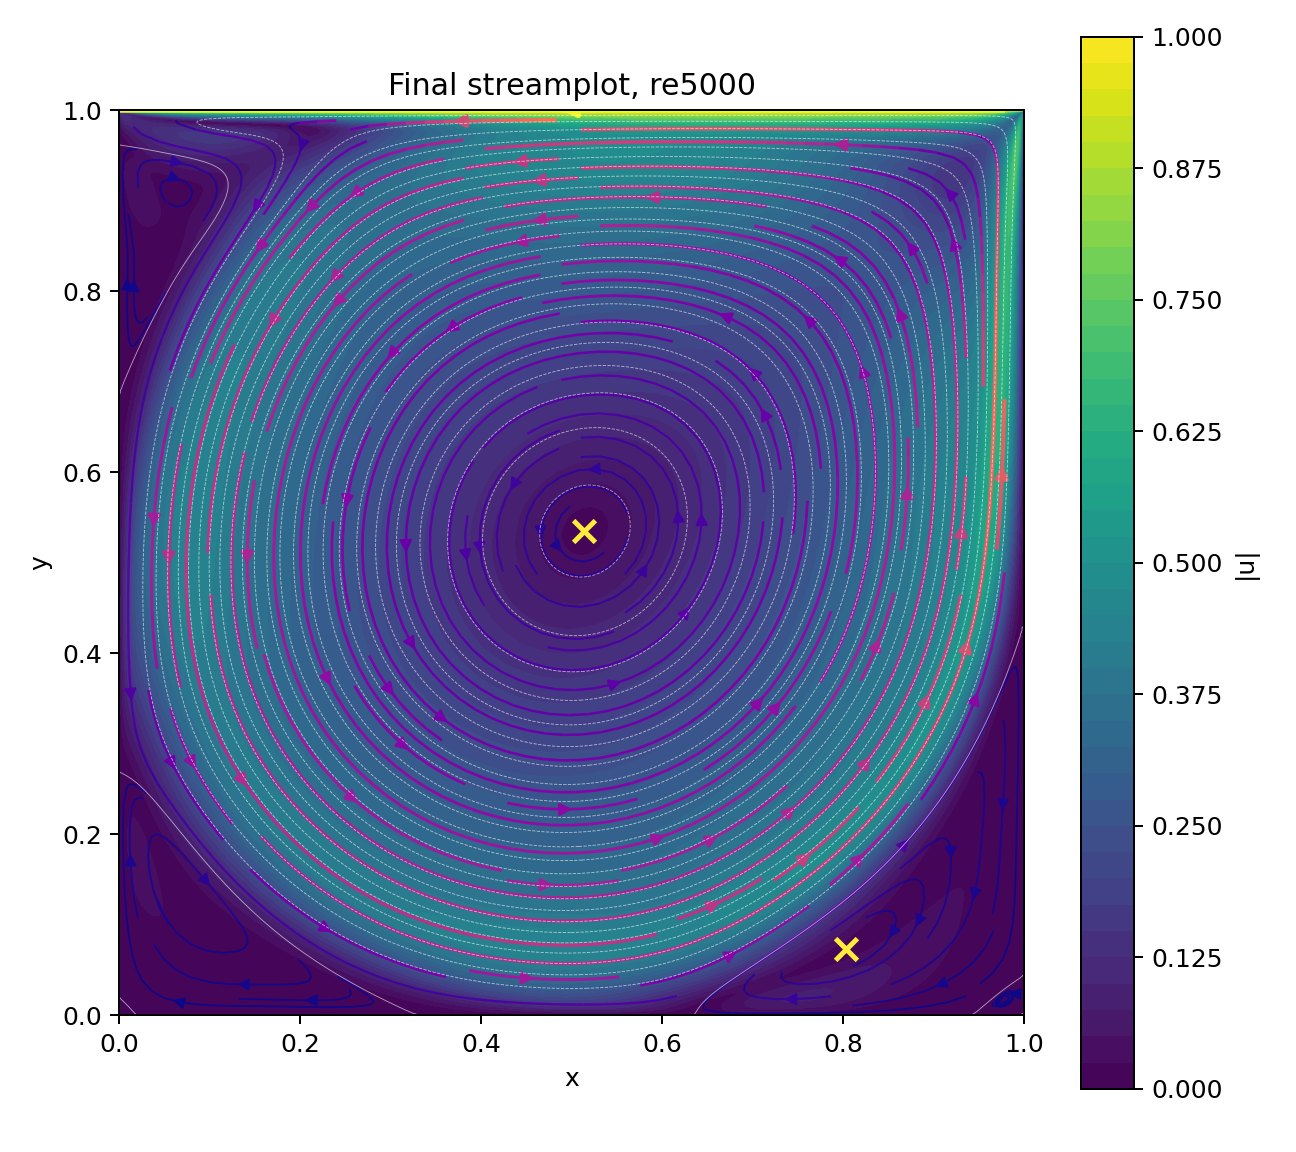
\includegraphics[width=\textwidth]{images/cavity_re5000_streamplot.png}
        \caption{\(\Reynolds=5000\)}
    \end{subfigure}
    \begin{subfigure}{0.32\textwidth}
        \centering
        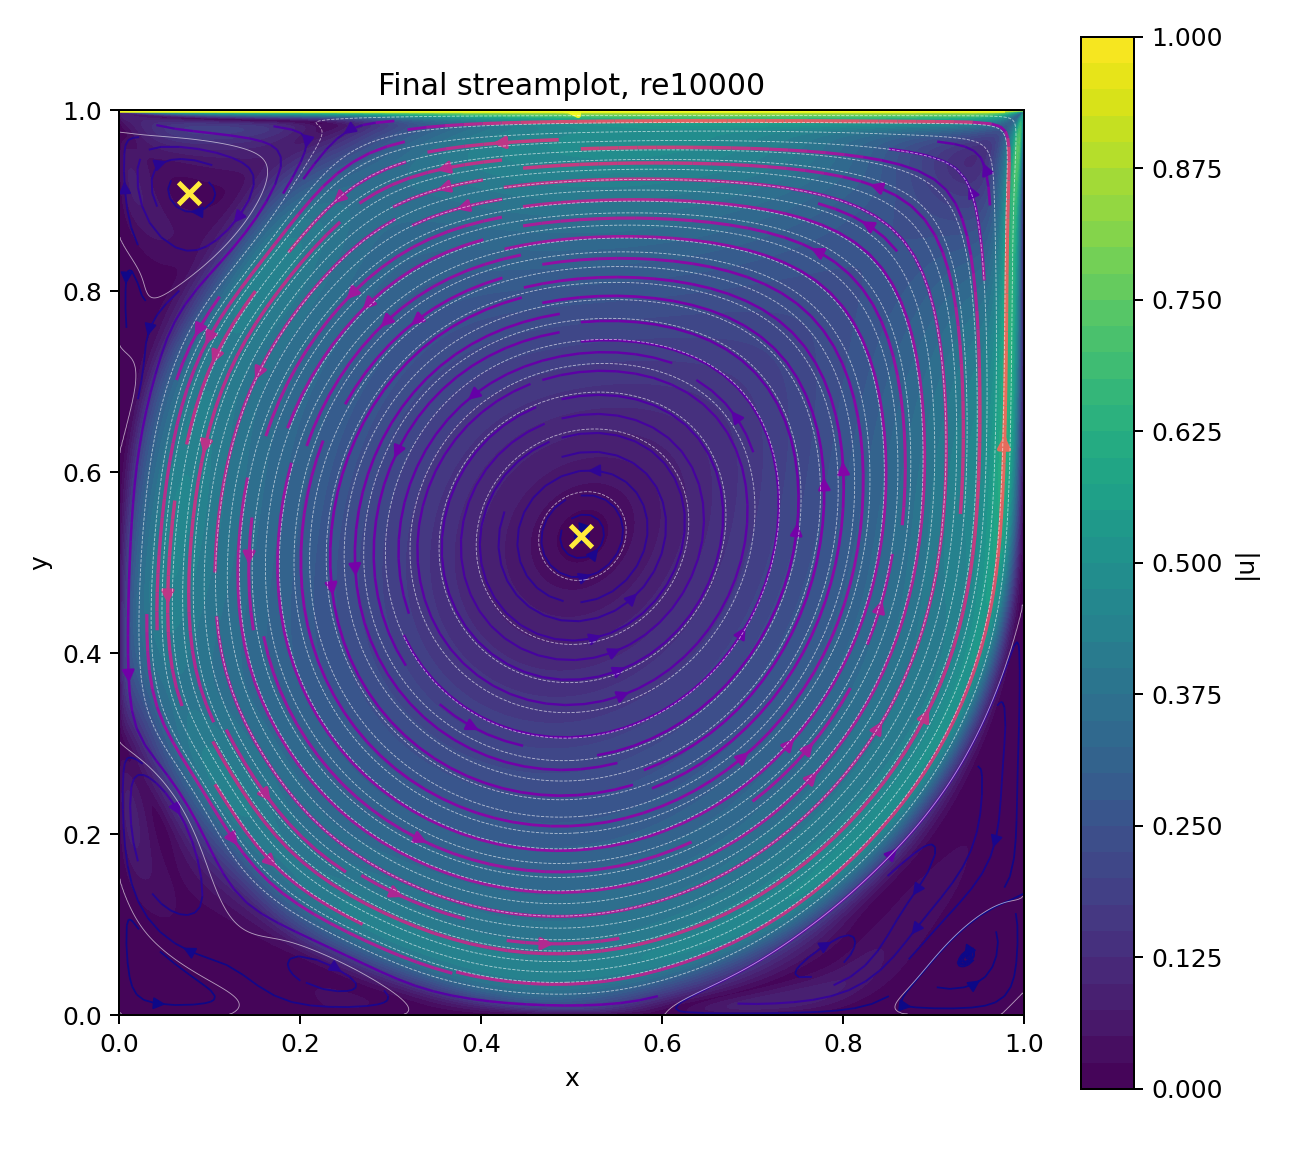
\includegraphics[width=\textwidth]{images/cavity_re10000_streamplot.png}
        \caption{\(\Reynolds=10000\)}
    \end{subfigure}
    \caption{Линии тока в квадратной каверне на сетке \(601\times601\). Жёлтыми крестами отмечены экстремумы функции тока, то есть центры наиболее выраженных вихревых ячеек. При росте \(\Reynolds\) главный вихрь смещается к геометрическому центру, а угловые вторичные вихри становятся заметнее.}
    \label{fig:cavity-streamplots-601}
\end{figure}

Количественная проверка удобно проводится по положению центров вихрей.
В~\cite{erturk2005} эти координаты приведены в таблице V для расчётов на сетке \(601\times601\).
Центры главного вихря в расчёте практически совпадают с табличными значениями.

\begin{table}[H]
    \centering
    \caption{Сравнение центра главного вихря в каверне с таблицей V из~\cite{erturk2005}.}
    \label{tab:cavity-primary-centers}
    \small
    \resizebox{\textwidth}{!}{%
    \begin{tabular}{@{}ccccc@{}}
        \toprule
        \(\Reynolds\) &
        \(\psi_{\min}\) в расчёте &
        \((x,y)\) в расчёте &
        \((x,y)\) из~\cite{erturk2005} &
        \(\psi\) из~\cite{erturk2005} \\
        \midrule
        1000  & \(-0.118776\) & \((0.5300,\,0.5650)\) & \((0.5300,\,0.5650)\) & \(-0.118781\) \\
        5000  & \(-0.121211\) & \((0.5150,\,0.5350)\) & \((0.5150,\,0.5350)\) & \(-0.121289\) \\
        10000 & \(-0.116012\) & \((0.5117,\,0.5300)\) & \((0.5117,\,0.5300)\) & \(-0.120403\) \\
        \bottomrule
    \end{tabular}
    }
\end{table}

Для \(\Reynolds=1000\) и \(\Reynolds=5000\) совпадает не только положение главного вихря, но и положение наиболее сильного вторичного вихря у нижнего правого угла:
\[
    (0.8633,0.1117),
    \qquad
    (0.8050,0.0733).
\]
Эти точки совпадают с центрами \(BR1\), указанными в~\cite{erturk2005}.
При \(\Reynolds=10000\) наиболее выраженный положительный экстремум в сохранённом снимке находится в верхнем углу:
\[
    (0.0783,0.9083),
\]
что соответствует области верхнего левого вторичного вихря \(TL1\) из таблицы V.

Таким образом, серия расчётов воспроизводит основные ориентиры из статьи: положение главного вихря, появление вторичных угловых вихрей и утончение пограничных слоёв.
Наибольшее расхождение по значению \(\psi_{\min}\) видно при \(\Reynolds=10000\).
Это ожидаемо: при больших \(\Reynolds\) стационарная каверна становится чувствительнее к времени интегрирования, сеточной диссипации и точности разрешения угловых вихрей, тогда как положение центра остаётся более устойчивой характеристикой.

\section{Эксперимент с четырьмя вихрями и задача стабилизации}

\subsection{Постановка в переменных \texorpdfstring{\((\psi,\omega)\)}{psi, omega}}

Второй вычислительный эксперимент посвящён форсированному течению в прямоугольной ячейке
\begin{equation}
    \Omega=(0,L_x)\times(0,L_y),
    \qquad
    L_x=1,\quad L_y=0.5.
    \label{eq:kornev-domain}
\end{equation}
Эта постановка мотивирована задачей о четырёхвихревой структуре из работы~\cite{kornev2018}, но далее она сразу записывается в тех переменных, в которых построен разностный алгоритм.
На границе ячейки задаётся
\begin{equation}
    \psi\big|_{\partial\Omega}=0,
    \label{eq:kornev-psi-wall}
\end{equation}
что соответствует непроницаемым стенкам; тангенциальная скорость стенок в текущем расчёте равна нулю.

Коэффициент вязкости обозначается через \(\nu\), а число Рейнольдса записывается только как
\begin{equation}
    \Reynolds=\frac{1}{\nu}.
    \label{eq:kornev-re-nu}
\end{equation}
В выполненном расчёте \(\Reynolds=1/\nu=260\), то есть \(\nu=1/260\).

Эволюционная система имеет вид
\begin{equation}
\begin{aligned}
    \psi_t
    &=
    \Laplace\psi+\omega,\\
    \omega_t
    &=
    \nu\Laplace\omega
    -
    \left(\psi_x\omega_y-\psi_y\omega_x\right)
    -
    F_\omega(x,y),
\end{aligned}
\label{eq:kornev-pseudo-system}
\end{equation}
Здесь \(F_\omega\) --- завихренная часть внешнего воздействия в соглашении, принятом в программе.
Именно \(F_\omega\) создаёт в прямоугольнике четыре крупные вихревые ячейки.
В явном виде
\begin{equation}
    F_\omega(x,y)
    =
    \sum_{(m,n)\in\mathcal M}
    a_{mn}\frac{\pi n}{L_y}
    \sin\frac{\pi m x}{L_x}
    \sin\frac{\pi n y}{L_y}.
    \label{eq:omega-forcing}
\end{equation}
Здесь используются моды
\[
    \mathcal M=\{(2,2),(4,2),(6,2),(2,4),(1,3),(3,1)\},
\]
а коэффициенты равны
\begin{equation}
\begin{aligned}
    a_{22}&=-\frac{19L_y}{2\pi},&
    a_{42}&=-\frac{6L_y}{2\pi},&
    a_{62}&=\frac{7L_y}{2\pi},\\
    a_{24}&=\frac{14L_y}{4\pi},&
    a_{13}&=\frac{a_{22}}{50},&
    a_{31}&=\frac{a_{22}}{50}.
\end{aligned}
\label{eq:force-coefficients}
\end{equation}
Малые моды с коэффициентами \(a_{13}\) и \(a_{31}\) усиливают неустойчивость и ускоряют выход траектории на колебательный режим.

Стационарная система, к которой стремится псевдовременной процесс, имеет вид
\begin{equation}
\begin{aligned}
    \Laplace\psi+\omega&=0,\\
    \nu\Laplace\omega
    -
    \left(\psi_x\omega_y-\psi_y\omega_x\right)
    -
    F_\omega(x,y)&=0.
\end{aligned}
\label{eq:kornev-steady-system}
\end{equation}

В отличие от задачи о каверне, здесь нет движущейся стенки.
Течение создаётся объёмной завихренной силой \eqref{eq:omega-forcing}, а стенки только ограничивают область и задают условие прилипания.
Именно форма forcing-а приводит к четырёхвихревой структуре: синусоидальные моды возбуждают попеременно вращающиеся вихревые ячейки.

\subsection{Идея стабилизационного эксперимента}

Эксперимент строится вокруг неустойчивого четырёхвихревого стационара.
Сначала исходная система \eqref{eq:kornev-pseudo-system} интегрируется из нулевого состояния.
Траектория быстро приближается к четырёхвихревому режиму, но затем уходит от него, потому что этот режим имеет неустойчивые направления.
Поэтому прямое интегрирование используется не как окончательный способ поиска стационара, а как способ получить хорошее начальное приближение.

Дальше выполняются три связанных шага.
Во-первых, выбирается снимок, для которого относительная разность соседних состояний минимальна.
Во-вторых, это состояние уточняется методом Ньютона как решение нелинейной разностной системы \(F(U)=0\).
В-третьих, около найденного стационара строится линеаризованный оператор, находится его спектр и выделяются собственные моды с \(\operatorname{Re}\lambda>0\).
Именно эти моды отвечают росту возмущений и последующему разрушению почти стационарной четырёхвихревой картины.

Стабилизация в данной реализации выполняется как разностная проекция: из текущего состояния вычитается компонента, лежащая в вещественном подпространстве неустойчивых собственных мод.
В статье~\cite{kornev2018} аналогичная идея связана с проекцией на устойчивое многообразие и построением граничного управления.
Здесь же реализован более простой вычислительный вариант: граничные условия остаются нулевыми, а подавление неустойчивости проводится непосредственно в пространстве сеточных состояний.

\section{Разностная схема для эксперимента с четырьмя вихрями}

Сетка остаётся равномерной:
\[
    x_i=ih_x,\quad h_x=\frac{L_x}{N_x},
    \qquad
    y_j=jh_y,\quad h_y=\frac{L_y}{N_y}.
\]
В выполненном расчёте
\begin{equation}
    N_x+1=201,\qquad N_y+1=101,\qquad
    h_x=h_y=0.005.
    \label{eq:second-grid-size}
\end{equation}
Шаг по времени равен
\begin{equation}
    \tau=10^{-5}.
    \label{eq:second-dt}
\end{equation}

Лапласиан аппроксимируется оператором \eqref{eq:discrete-laplacian}.
Теперь нелинейный член аппроксимируется не простой центральной формулой, а схемой Аракавы.
С этого места удобно ввести обозначение
\begin{equation}
    J(\psi,\omega)
    =
    \psi_x\omega_y-\psi_y\omega_x.
    \label{eq:jacobian-definition}
\end{equation}
Его разностный аналог строится как усреднение трёх форм:
\begin{equation}
    J_h^A(\psi,\omega)
    =
    \frac13\left(J_h^{(1)}+J_h^{(2)}+J_h^{(3)}\right),
    \label{eq:arakawa}
\end{equation}
где \(J_h^{(1)}\) --- обычный центральный якобиан, а \(J_h^{(2)}\) и \(J_h^{(3)}\) --- две эквивалентные дискретные формы, полученные переносом разностей на множители.
Смысл такого усреднения состоит в том, что для невязкого переноса схема лучше сохраняет дискретные аналоги энергии и энстрофии, поэтому ведёт себя физичнее на длинной динамике.
Это особенно важно в эксперименте с четырьмя вихрями: дальнейший спектральный анализ чувствителен к тому, насколько аккуратно разностная схема передаёт структуру стационарного состояния.

По времени используется та же идея псевдовременной факторизации, что и в первой задаче.
Уравнение для \(\psi\) решается через две прогонки по направлениям, а для \(\omega\) диффузионная часть учитывается неявно в факторизованном виде.
Правая часть для завихренности содержит уже рассчитанный \(J_h^A(\psi,\omega)\) и внешнее воздействие \(F_\omega\).
Схема имеет первый порядок по времени и второй порядок по пространству во внутренних узлах; \(J_h^A\) также использует симметричный девятиточечный шаблон второго порядка.

Граничные условия для функции тока однородные:
\begin{equation}
    \psi\big|_{\partial\Omega}=0.
    \label{eq:second-psi-bc}
\end{equation}
Так как все стенки неподвижны, формула Тома принимает вид
\begin{equation}
\begin{aligned}
    \omega_{i,0}
    &=-\frac{2\psi_{i,1}}{h_y^2},&
    \omega_{i,N_y}
    &=-\frac{2\psi_{i,N_y-1}}{h_y^2},\\
    \omega_{0,j}
    &=-\frac{2\psi_{1,j}}{h_x^2},&
    \omega_{N_x,j}
    &=-\frac{2\psi_{N_x-1,j}}{h_x^2}.
\end{aligned}
\label{eq:second-thom}
\end{equation}

\section{Реализация и результаты четырёхвихревого эксперимента}

Основное состояние расчёта состоит из полей
\[
    x,\ y,\ \psi,\ \omega,\ u,\ v,
\]
то есть из координат сетки, функции тока, завихренности и двух компонент скорости.
В текущей структуре проекта основные снимки записываются в бинарном формате, а служебные таблицы --- например история невязок, спектр и список выбранных снимков --- остаются в CSV.
Для рисунков в этом разделе использованы те же величины \((x,y,\psi,\omega,u,v)\), восстановленные на сетке \(201\times101\).
Внутри одного шага сначала обновляется функция тока, затем граничная завихренность, затем поле \(\omega\), после чего вычисляются скорости и стационарные невязки.
Сохранение выполняется каждые \(1000\) шагов, поэтому временной интервал между соседними снимками равен \(10^{-2}\).

\begin{figure}[H]
    \centering
    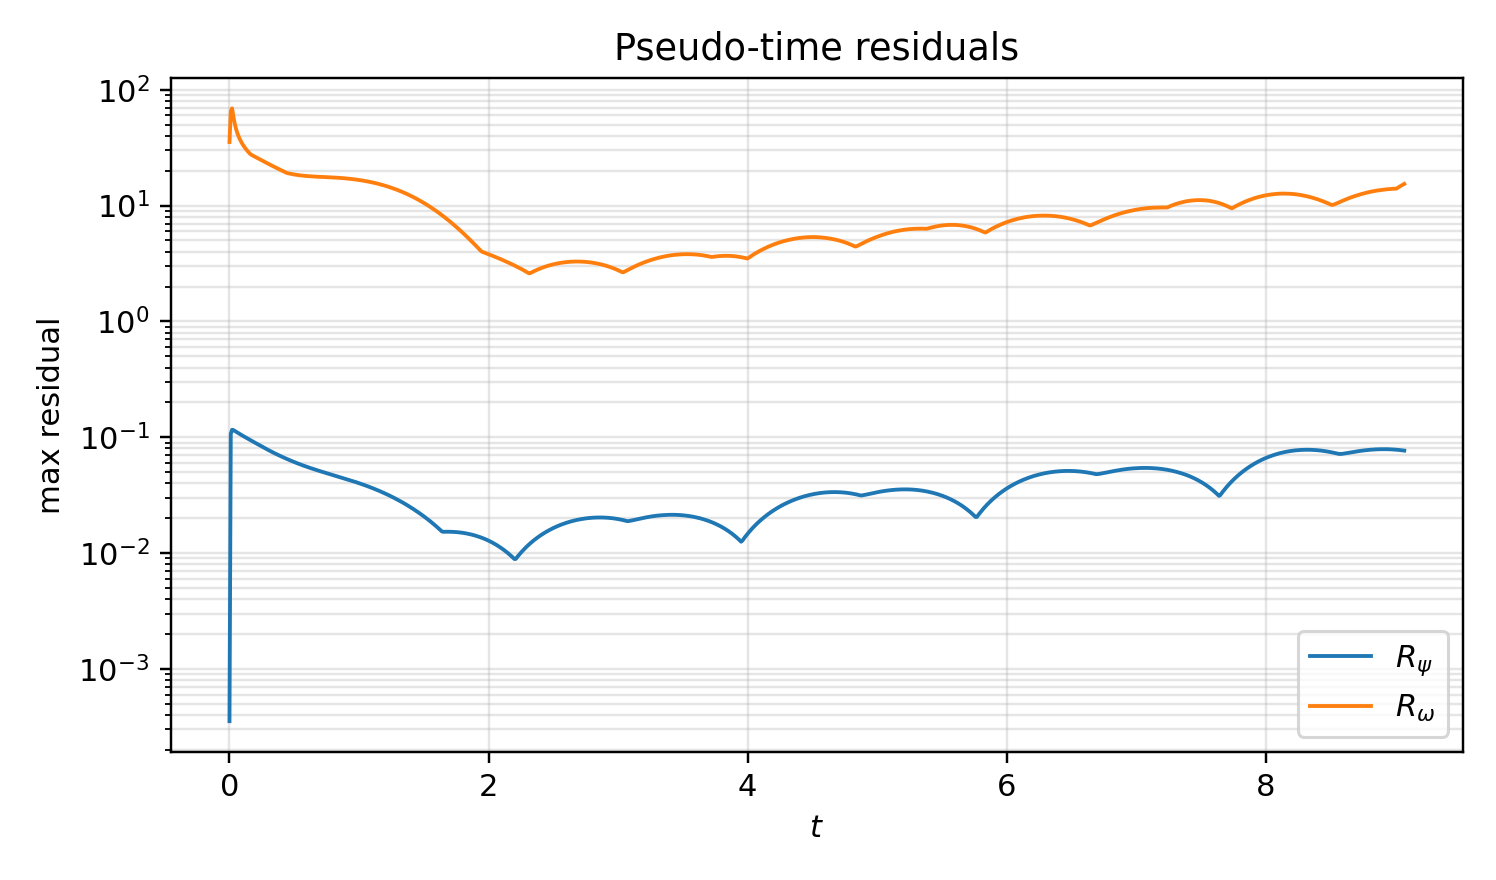
\includegraphics[width=0.82\textwidth]{images/residual_history.png}
    \caption{История псевдовременных невязок \(R_\psi\) и \(R_\omega\) для четырёхвихревого эксперимента. График показывает, что решение быстро выходит из нулевого состояния в режим, где стационарная невязка уже не убывает монотонно: это связано с приближением к неустойчивому стационарному состоянию и последующим уходом от него.}
    \label{fig:residual-history}
\end{figure}

Для поиска почти стационарного состояния сравнивались соседние сохранённые снимки.
Если \(U_k=(\psi_k,\omega_k)\), то использовалась относительная величина
\begin{equation}
    D_k=
    \frac{\norm{U_k-U_{k-1}}_2}{\norm{U_k}_2}.
    \label{eq:consecutive-difference}
\end{equation}
Минимум в исходной последовательности достигается между шагами \(235000\) и \(236000\), то есть при \(t=2.36001\):
\[
    D_{\min}=1.06\cdot10^{-3}
    \quad\text{после округления}.
\]

\begin{figure}[H]
    \centering
    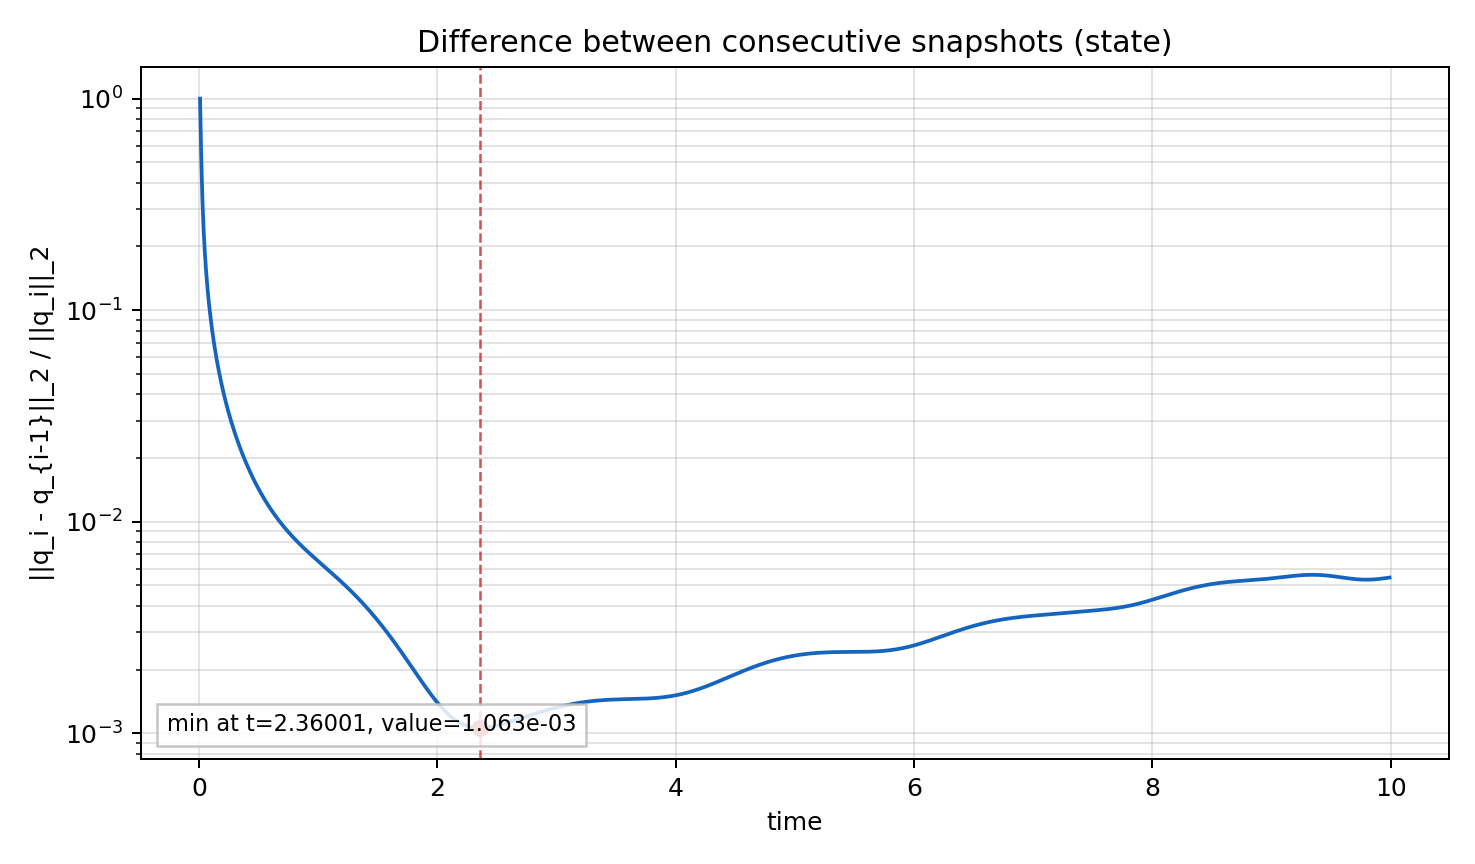
\includegraphics[width=0.82\textwidth]{images/stationary_consecutive_difference.png}
    \caption{Относительная разность соседних снимков в исходном расчёте. Быстрое убывание в начале означает приближение к четырёхвихревому режиму, а последующий рост показывает уход траектории вдоль неустойчивого направления.}
    \label{fig:stationary-consecutive}
\end{figure}

\begin{figure}[H]
    \centering
    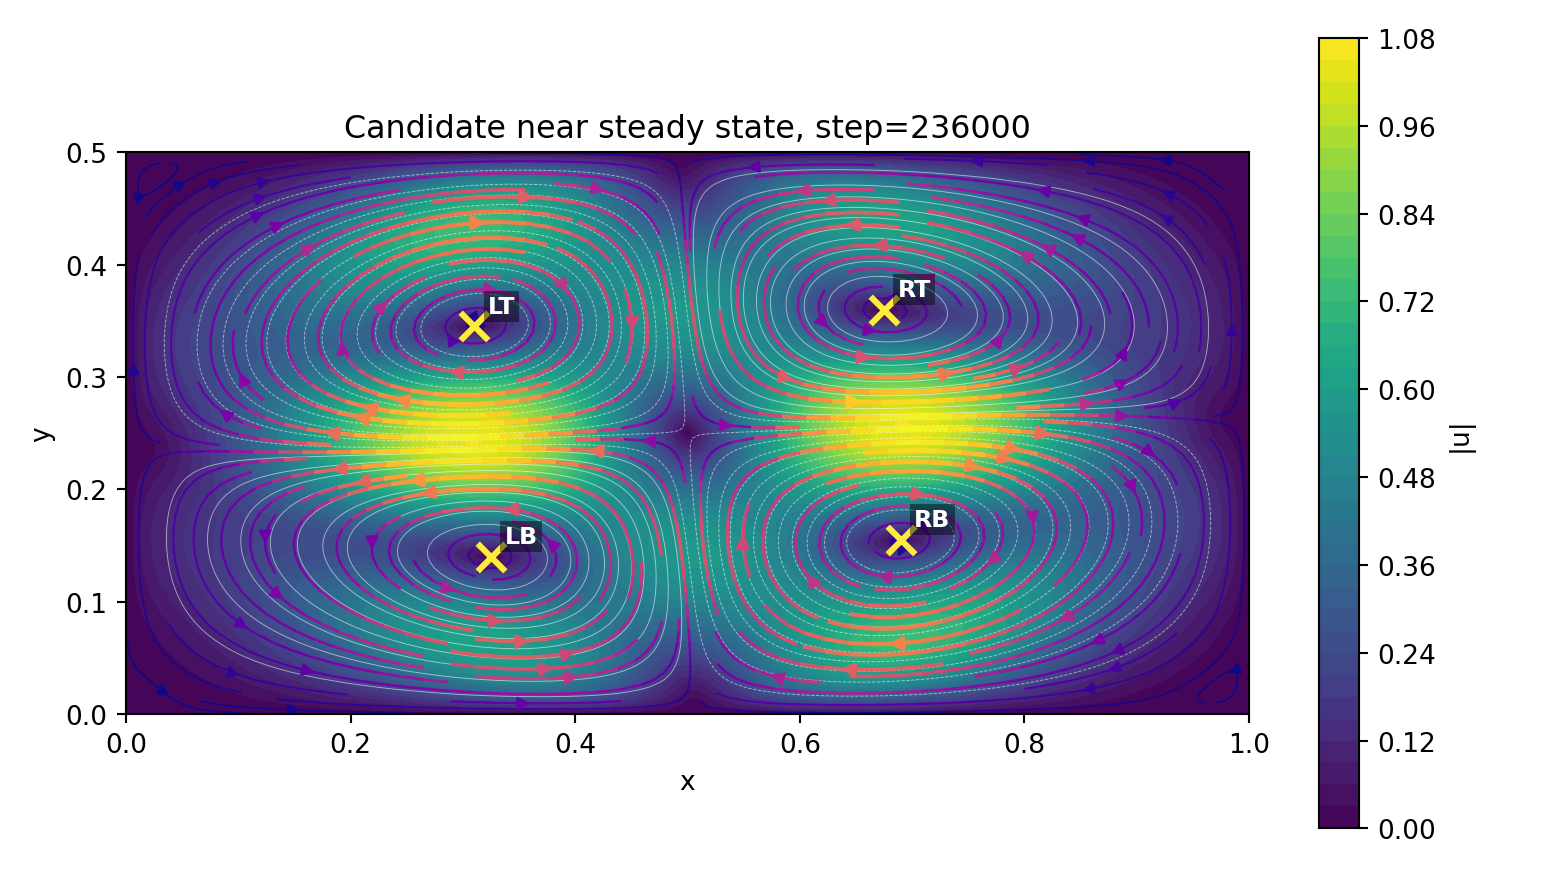
\includegraphics[width=0.88\textwidth]{images/pulsation_candidate_centers.png}
    \caption{Линии тока для кандидата в стационарное состояние при \(t=2.36001\). Жёлтыми крестами отмечены центры четырёх вихрей, найденные как доминирующие экстремумы \(\psi\) в четырёх геометрических ячейках области. Видна структура, характерная для форсировки \eqref{eq:omega-forcing}: в прямоугольнике формируются четыре крупные ячейки с чередующимся направлением вращения.}
    \label{fig:stationary-candidate}
\end{figure}

В работе~\cite{kornev2018} координаты центров вихрей не приведены отдельной таблицей.
Поэтому для численного сравнения я использую геометрические центры четырёх ячеек магнитной структуры \(2\times2\), соответствующей рисунку 1 из~\cite{kornev2018}:
\[
    (0.25,0.125),\quad
    (0.75,0.125),\quad
    (0.25,0.375),\quad
    (0.75,0.375).
\]
Это не табличный benchmark, как в задаче о каверне, а ориентир, показывающий, где должна располагаться четырёхвихревая шахматная структура.
В вычисленном кандидате центры заметно смещены от этих геометрических точек к внутренним разделительным слоям, где скорость максимальна.
Такое смещение естественно: центры вихрей определяются не только расположением гармоник forcing-а, но и вязкостью, условием прилипания на стенках и нелинейным переносом.

\begin{table}[H]
    \centering
    \caption{Координаты центров четырёх вихрей в задаче пульсации. Колонка из~\cite{kornev2018} содержит геометрические ориентиры по рисунку 1, а не таблично измеренные координаты.}
    \label{tab:pulsation-vortex-centers}
    \small
    \resizebox{\textwidth}{!}{%
    \begin{tabular}{@{}ccccc@{}}
        \toprule
        Ячейка &
        ориентир из~\cite{kornev2018} &
        кандидат \(t=2.36001\) &
        исходная динамика \(t=10\) &
        после фильтрации \(t=10\) \\
        \midrule
        LB & \((0.250,\,0.125)\) & \((0.325,\,0.140)\) & \((0.260,\,0.245)\) & \((0.300,\,0.145)\) \\
        RB & \((0.750,\,0.125)\) & \((0.690,\,0.155)\) & \((0.715,\,0.175)\) & \((0.690,\,0.155)\) \\
        LT & \((0.250,\,0.375)\) & \((0.310,\,0.345)\) & \((0.285,\,0.325)\) & \((0.310,\,0.345)\) \\
        RT & \((0.750,\,0.375)\) & \((0.675,\,0.360)\) & \((0.740,\,0.255)\) & \((0.700,\,0.355)\) \\
        \bottomrule
    \end{tabular}
    }
\end{table}

Таблица показывает смысл пульсационного режима.
Вблизи почти стационарного состояния четыре центра расположены симметрично: нижняя левая и верхняя правая ячейки имеют положительную функцию тока, а нижняя правая и верхняя левая --- отрицательную.
К моменту \(t=10\) исходная динамика уже нарушает эту структуру: центры LB и RT уходят к центральной горизонтальной линии, что соответствует началу диагональной перестройки вихрей.
После вычитания неустойчивой компоненты центры снова оказываются близки к четырёхвихревому кандидату.

После уточнения методом Ньютона получено стационарное состояние, у которого
\[
    \min\psi=-0.06964,\quad
    \max\psi=0.06222,\quad
    \min\omega=-25.0093,\quad
    \max\omega=26.0354.
\]
Максимальные скорости по модулю в сохранённом состоянии составляют
\[
    |u|_{\max}=1.0431,\qquad |v|_{\max}=0.5634
    \quad \text{после округления}.
\]

\begin{figure}[H]
    \centering
    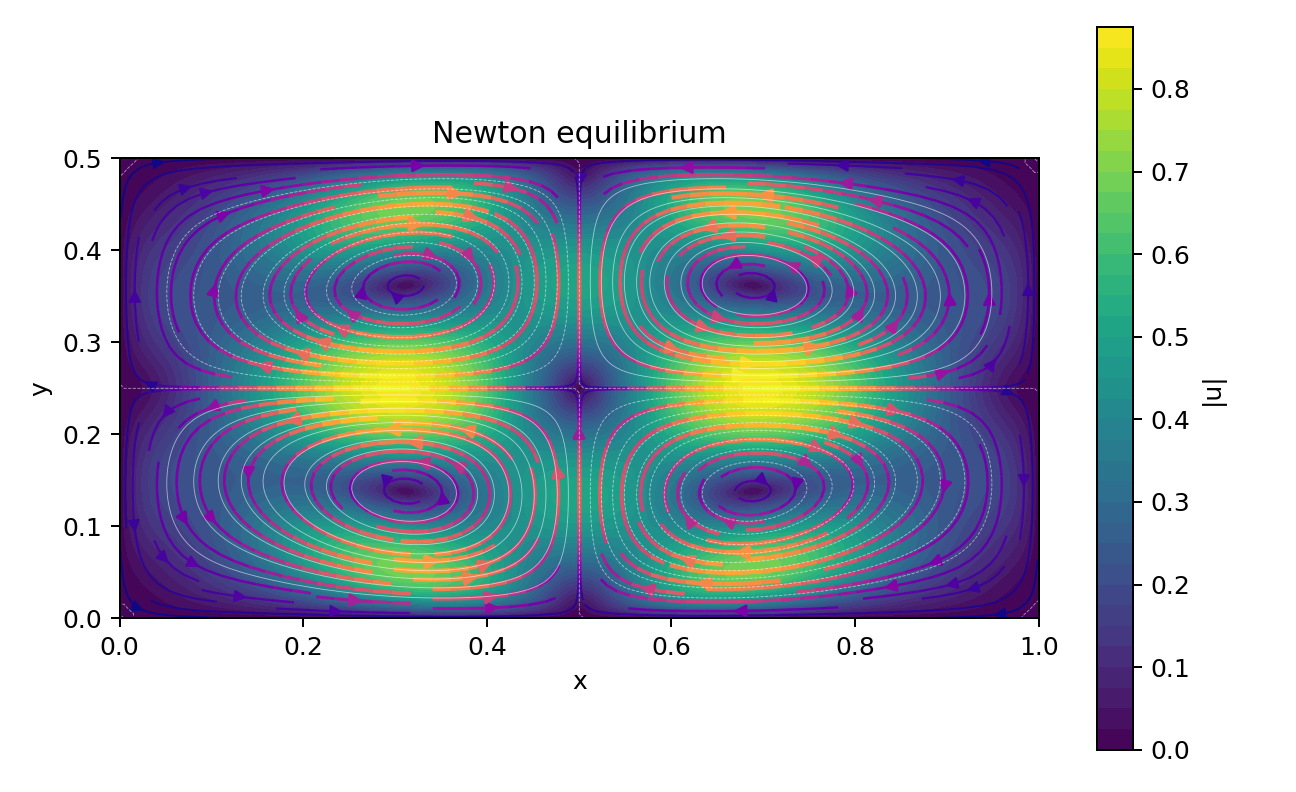
\includegraphics[width=0.82\textwidth]{images/newton_equilibrium_streamplot.png}
    \caption{Линии тока стационарного состояния после уточнения методом Ньютона. По сравнению с кандидатом из исходной эволюции структура становится более регулярной и симметричной, что соответствует решению нелинейной стационарной системы \eqref{eq:kornev-steady-system}.}
    \label{fig:newton-equilibrium-streamplot}
\end{figure}

\begin{figure}[H]
    \centering
    \begin{subfigure}{0.49\textwidth}
        \centering
        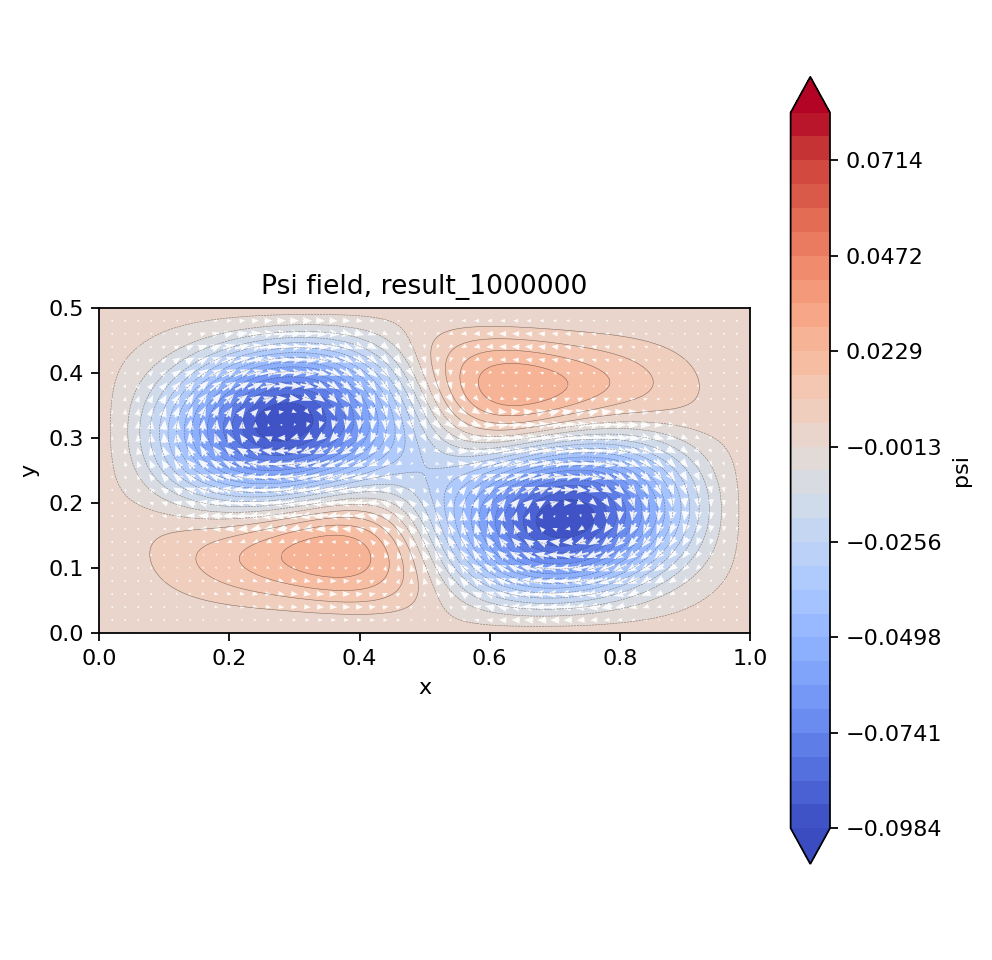
\includegraphics[width=\textwidth]{images/raw_result_1000000_psi.png}
        \caption{\(\psi\)}
    \end{subfigure}
    \begin{subfigure}{0.49\textwidth}
        \centering
        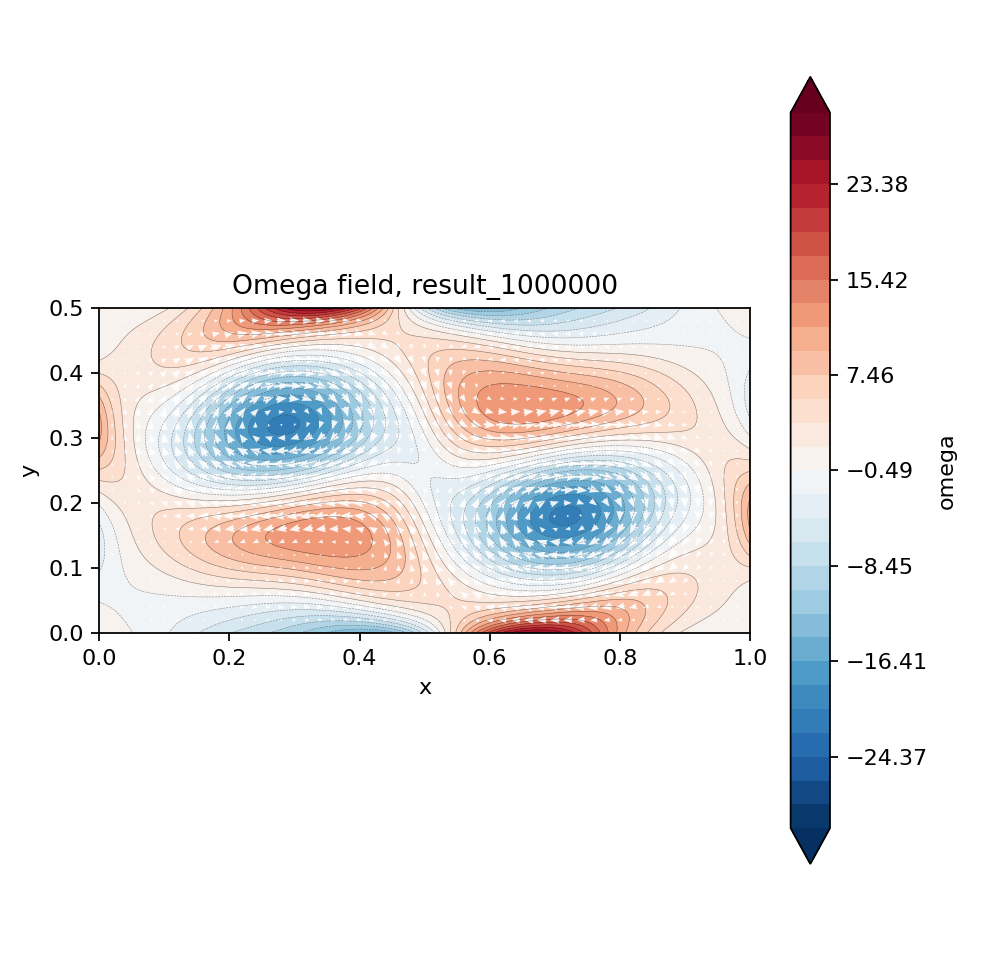
\includegraphics[width=\textwidth]{images/raw_result_1000000_omega.png}
        \caption{\(\omega\)}
    \end{subfigure}
    \caption{Поля функции тока и завихренности в исходной динамике на шаге \(10^6\). Нарушение симметрии по сравнению с \cref{fig:newton-equilibrium-streamplot} показывает, что траектория ушла от неустойчивого стационара.}
    \label{fig:raw-fields}
\end{figure}

\begin{figure}[H]
    \centering
    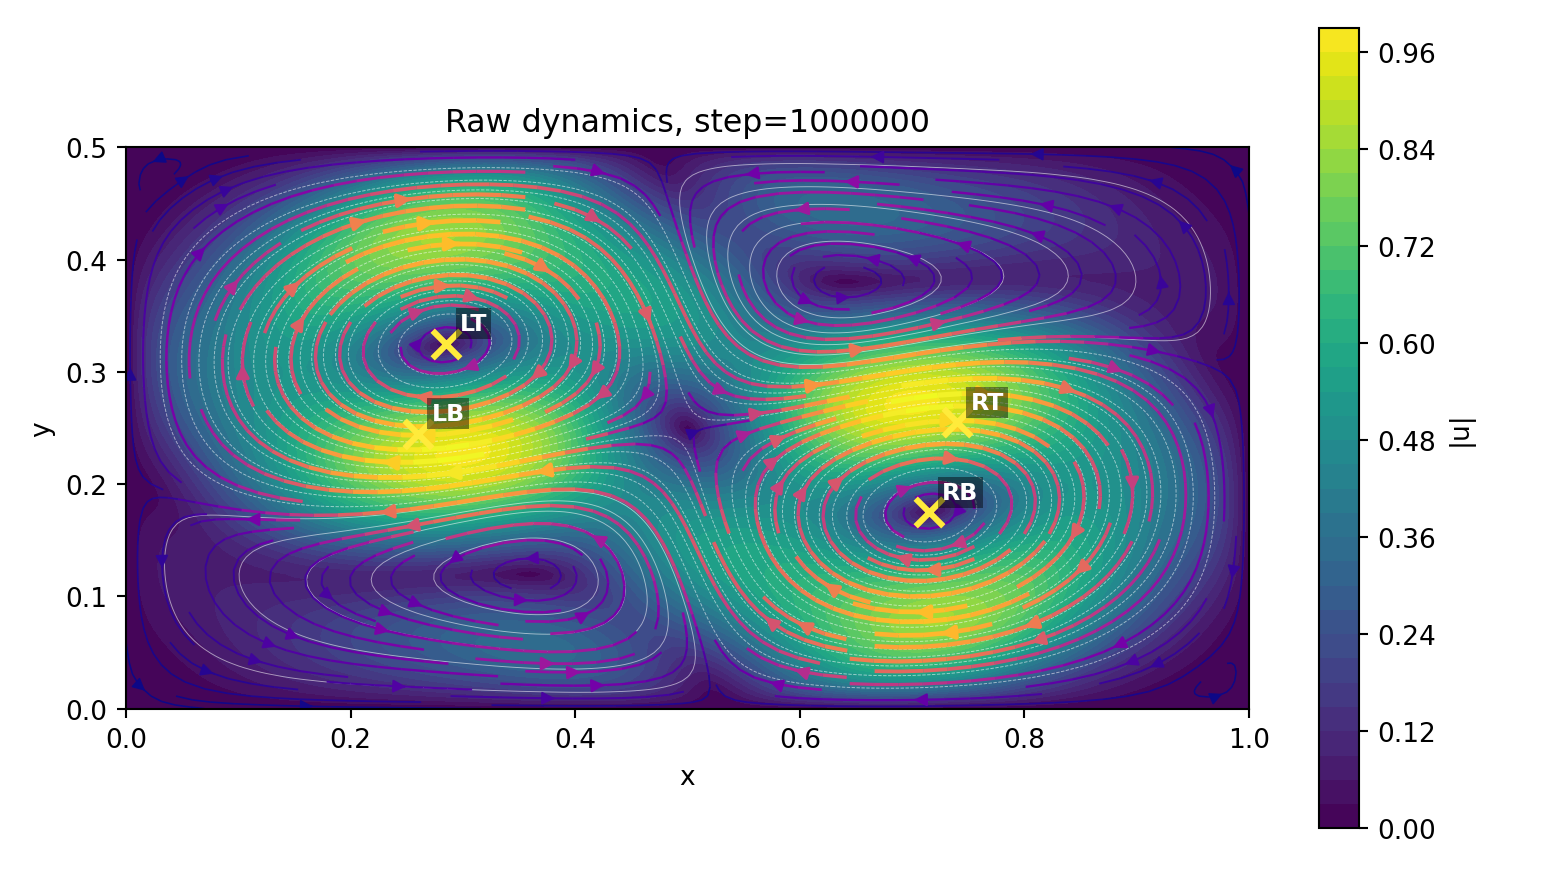
\includegraphics[width=0.88\textwidth]{images/pulsation_raw_1000000_centers.png}
    \caption{Линии тока исходного решения на шаге \(10^6\), то есть при \(t=10\). Картина уже не является чисто четырёхвихревой: центры двух диагональных ячеек смещаются к середине области, и начинается перестройка к колебательному режиму, описанному в~\cite{kornev2018}.}
    \label{fig:raw-streamplot}
\end{figure}

\section{Поиск стационарного решения}

Стационарное решение четырёхвихревого эксперимента определяется системой
\begin{equation}
    F(U)=0,
    \qquad
    U=(\psi,\omega).
    \label{eq:stationary-operator}
\end{equation}
После дискретизации \(U\) становится большим вектором внутренних сеточных значений.
Если внутренних узлов \(N=(N_x-1)(N_y-1)\), то используется упаковка
\begin{equation}
    U=
    \left(
    \psi_{1,1},\ldots,\psi_{N_x-1,N_y-1},
    \omega_{1,1},\ldots,\omega_{N_x-1,N_y-1}
    \right)^T.
    \label{eq:state-packing}
\end{equation}
Двумерные индексы переводятся в одномерный номер обычной построчной нумерацией.
Граничные значения \(\psi\) не входят в вектор неизвестных, потому что они равны нулю.
Граничные значения \(\omega\) также не являются независимыми: они восстанавливаются из \(\psi\) по формуле Тома \eqref{eq:second-thom}.

Оператор \(F(U)\) имеет две группы компонент:
\begin{equation}
    F(U)=
    \begin{pmatrix}
    \Laplace_h\psi+\omega\\
    \nu\Laplace_h\omega
    -J_h^A(\psi,\omega)-F_\omega
    \end{pmatrix}.
    \label{eq:discrete-stationary-residual}
\end{equation}
Первая группа отвечает дискретному уравнению Пуассона, вторая --- стационарному балансу диффузии, переноса и внешнего forcing-а.
В качестве начального приближения для Ньютона берётся снимок, для которого величина \eqref{eq:consecutive-difference} минимальна.
Такой выбор важен: неустойчивый стационар может быть недостижим как предел прямого интегрирования, но траектория проходит достаточно близко к нему, чтобы метод Ньютона смог уточнить решение.

\section{Метод Ньютона}

Для нелинейной системы \eqref{eq:stationary-operator} применяется метод Ньютона:
\begin{equation}
\begin{aligned}
    J_F(U^k)\delta U^k&=-F(U^k),\\
    U^{k+1}&=U^k+\alpha_k\delta U^k.
\end{aligned}
\label{eq:newton}
\end{equation}
Здесь \(J_F(U^k)\) --- якобиан дискретного оператора \(F\), а \(\alpha_k\in(0,1]\) --- параметр демпфирования.
Он выбирается простым поиском по шагу: если полная поправка не уменьшает \(L^2\)-норму невязки, \(\alpha_k\) последовательно делится пополам.

Якобиан явно не собирается.
Вместо этого реализовано произведение \(V\mapsto J_F(U)V\).
Для возмущения \(V=(\phi,\eta)\) линейная часть имеет вид
\begin{equation}
    J_F(U)
    \begin{pmatrix}
    \phi\\ \eta
    \end{pmatrix}
    =
    \begin{pmatrix}
    \Laplace_h\phi+\eta\\
    \nu\Laplace_h\eta
    -J_h^A(\phi,\omega)
    -J_h^A(\psi,\eta)
    \end{pmatrix}.
    \label{eq:newton-jv}
\end{equation}
Линейная система в \eqref{eq:newton} решается методом GMRES.
В качестве предобуславливателя используется стоксово приближение: обратный дискретный лапласиан с нулевыми условиями Дирихле применяется через синус-преобразование.
Это согласуется с геометрией прямоугольника и однородным условием \(\psi=0\) на границе.

Сходимость контролируется двумя нормами.
Для остановки Ньютона используется максимум по компонентам,
\begin{equation}
    \norm{F(U^k)}_\infty,
    \label{eq:newton-linf}
\end{equation}
а для выбора демпфирующего шага --- среднеквадратичная норма невязки.
Отдельный график сходимости Ньютона в переданных результатах не сохранён; для окончательной версии отчёта его следует восстановить из лога повторного запуска.

\begin{figure}[H]
    \centering
    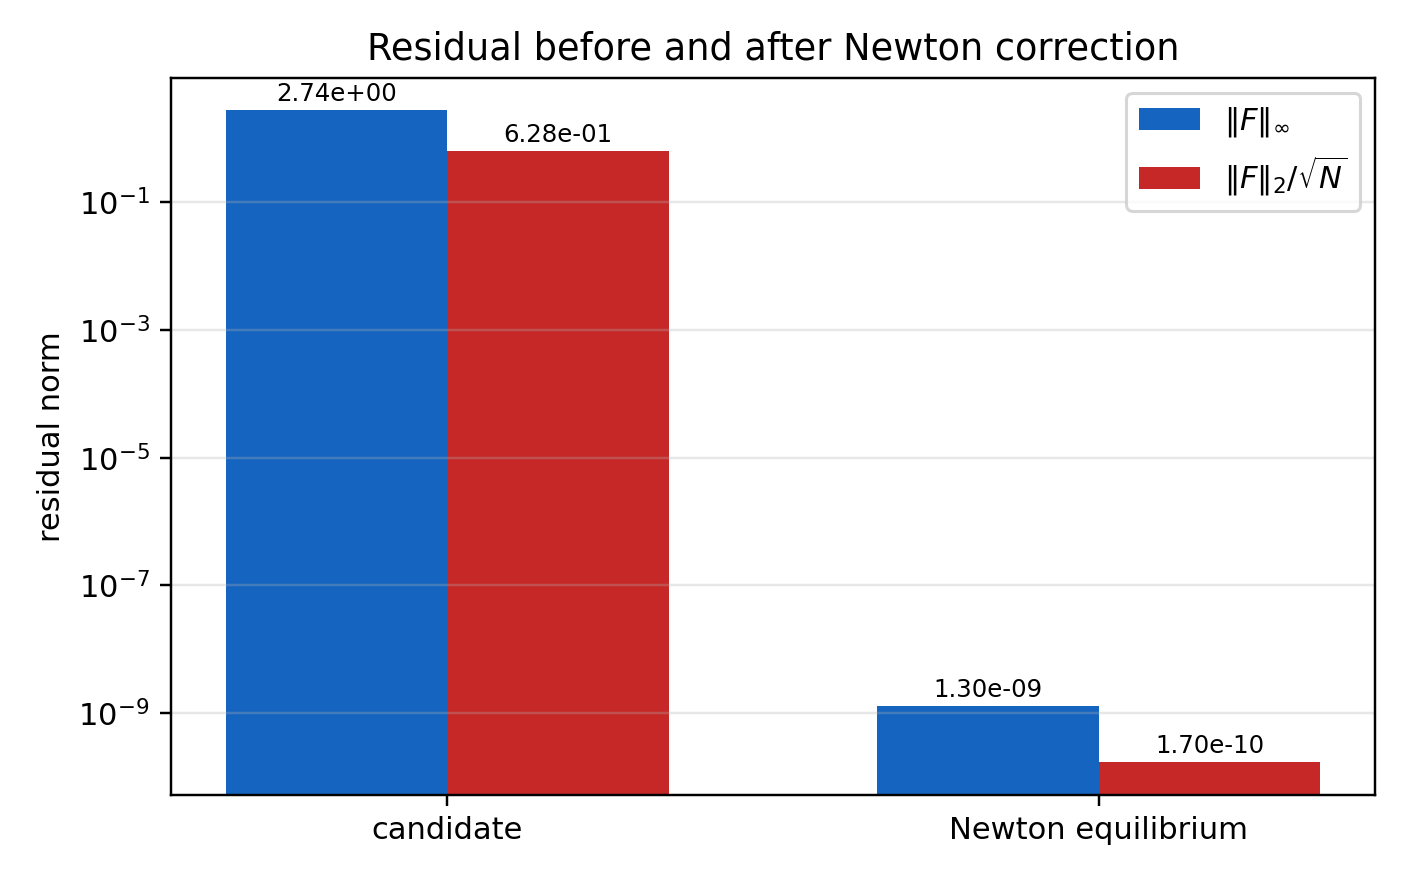
\includegraphics[width=0.74\textwidth]{images/newton_residual_drop.png}
    \caption{Невязка стационарной системы \eqref{eq:discrete-stationary-residual} до и после ньютоновского уточнения. Для кандидата из прямого интегрирования \(\norm{F}_\infty=2.74\), после метода Ньютона \(\norm{F}_\infty=1.30\cdot10^{-9}\).}
    \label{fig:newton-residual-drop}
\end{figure}

\section{Линеаризация и спектральный анализ}

Пусть \(U_*=(\psi_*,\omega_*)\) --- стационарное решение, найденное методом Ньютона.
Рассмотрим малое возмущение
\begin{equation}
    \psi=\psi_*+\phi,\qquad
    \omega=\omega_*+\eta.
    \label{eq:perturbation}
\end{equation}
Подстановка \eqref{eq:perturbation} в эволюционную систему \eqref{eq:kornev-pseudo-system} и отбрасывание квадратичных членов даёт
\begin{equation}
\begin{aligned}
    \Laplace\phi+\eta&=0,\\
    \eta_t
    &=
    \nu\Laplace\eta
    -
    J(\phi,\omega_*)
    -
    J(\psi_*,\eta).
\end{aligned}
\label{eq:linearized-system}
\end{equation}
Из первого уравнения \(\phi\) восстанавливается по \(\eta\):
\begin{equation}
    \phi=-\Laplace^{-1}\eta,
    \label{eq:phi-from-eta}
\end{equation}
где обратный лапласиан понимается с нулевыми условиями Дирихле.
Поэтому линейная динамика может быть записана как одно уравнение для завихренности:
\begin{equation}
    \eta_t=\mathcal A\eta,
    \label{eq:eta-linear-evolution}
\end{equation}
где
\begin{equation}
    \mathcal A\eta
    =
    \nu\Laplace\eta
    -
    J(-\Laplace^{-1}\eta,\omega_*)
    -
    J(\psi_*,\eta).
    \label{eq:linearized-operator}
\end{equation}

Устойчивость стационара определяется спектром оператора \(\mathcal A\).
Ищутся собственные пары
\begin{equation}
    \mathcal A\varphi_k=\lambda_k\varphi_k.
    \label{eq:eigenproblem}
\end{equation}
Если \(\operatorname{Re}\lambda_k>0\), то возмущение \(e^{\lambda_k t}\varphi_k\) растёт экспоненциально.
В дискретной реализации матрица \(\mathcal A\) не собирается явно.
Для сетки \(201\times101\) число внутренних неизвестных для \(\eta\) равно
\[
    199\cdot99=19701,
\]
поэтому плотная матрица была бы слишком тяжёлой.
Используется матрично-свободный оператор: алгоритм Арнольди получает только действие \(\eta\mapsto\mathcal A\eta\).

В расчёте найдено \(30\) собственных значений с наибольшей действительной частью.
Неустойчивой оказалась одна комплексно-сопряжённая пара:
\begin{equation}
    \lambda_{0,1}
    =
    0.217011
    \pm
    1.786819\,i.
    \label{eq:unstable-eigenvalues}
\end{equation}
Действительная часть положительна, поэтому стационарное четырёхвихревое состояние является линейно неустойчивым.
Мнимая часть задаёт частоту колебаний:
\[
    \frac{|\operatorname{Im}\lambda|}{2\pi}=0.28438
    \quad \text{после округления}.
\]

\begin{figure}[H]
    \centering
    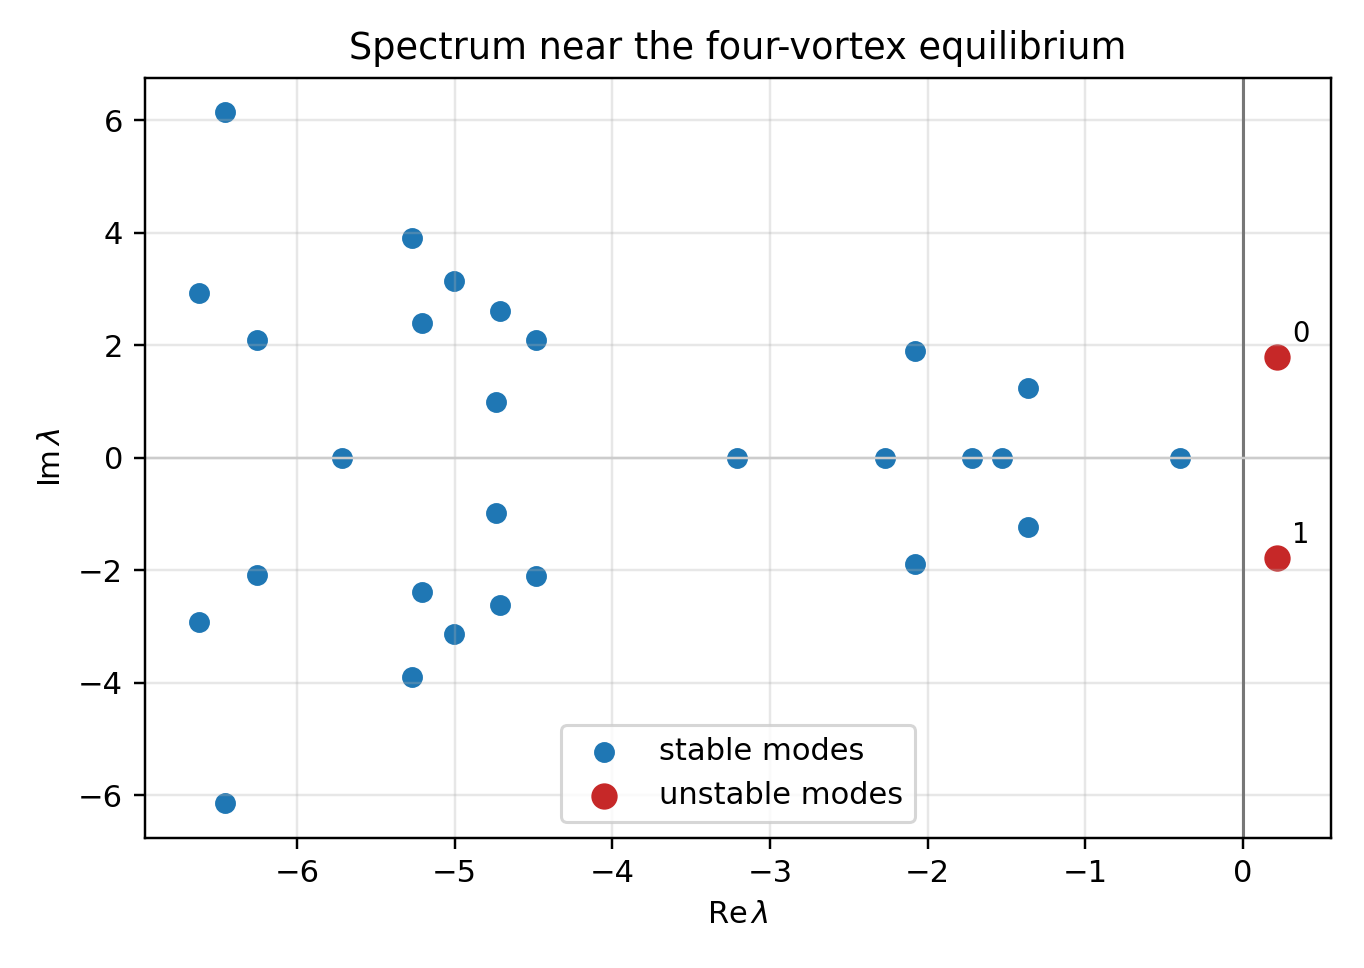
\includegraphics[width=0.82\textwidth]{images/stability_spectrum.png}
    \caption{Спектр линеаризованного оператора около четырёхвихревого стационара. Красным выделена комплексно-сопряжённая пара \eqref{eq:unstable-eigenvalues}; именно она отвечает росту возмущений и последующему уходу решения от стационарного режима.}
    \label{fig:stability-spectrum}
\end{figure}

\begin{figure}[H]
    \centering
    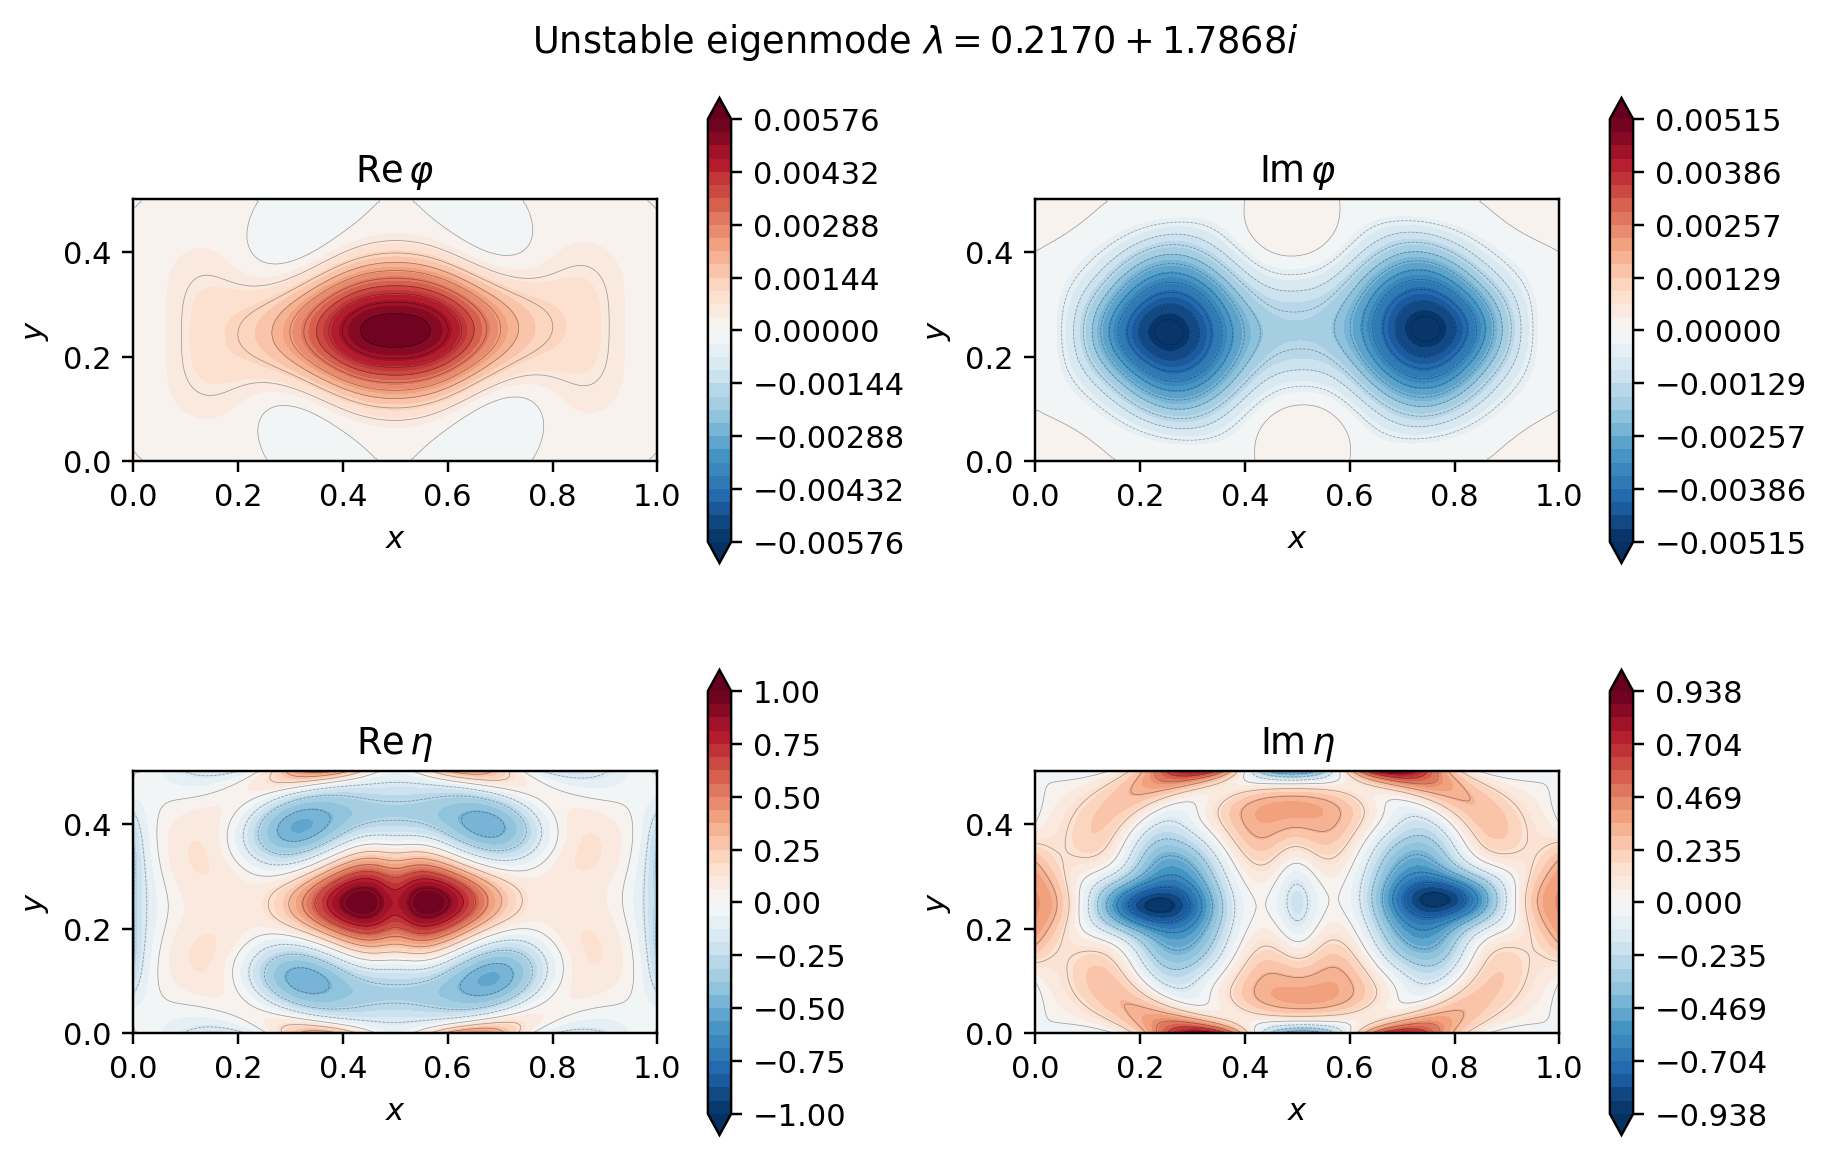
\includegraphics[width=0.96\textwidth]{images/unstable_mode_000.png}
    \caption{Вещественная и мнимая части неустойчивой собственной моды для \(\lambda=0.2170+1.7868i\) после округления. Верхний ряд показывает возмущение функции тока \(\phi\), нижний --- возмущение завихренности \(\eta\). Структура моды локализована так, что она перестраивает диагональные пары вихрей, вызывая переход к колебательному режиму.}
    \label{fig:unstable-mode}
\end{figure}

\section{Неустойчивые моды и стабилизация решения}

Линейная теория показывает, что в малой окрестности \(U_*\) наиболее опасна компонента возмущения, лежащая в подпространстве, натянутом на собственные векторы с \(\operatorname{Re}\lambda>0\).
Для комплексной моды
\[
    v=a+ib
\]
естественное вещественное неустойчивое подпространство имеет вид
\begin{equation}
    E_{\mathrm{unst}}
    =
    \operatorname{span}\{\operatorname{Re}v,\operatorname{Im}v\}.
    \label{eq:unstable-real-subspace}
\end{equation}
В коде полная мода хранится как пара \((\phi,\eta)\), то есть вектор состояния для проекции включает обе компоненты:
\begin{equation}
    q=
    \left(
    \phi_{1,1},\ldots,\phi_{N_x-1,N_y-1},
    \eta_{1,1},\ldots,\eta_{N_x-1,N_y-1}
    \right)^T.
    \label{eq:projection-state}
\end{equation}

Так как найденная пара комплексно-сопряжённая, достаточно взять одну комплексную моду и построить две вещественные функции.
Они ортонормируются модифицированным методом Грама--Шмидта в евклидовом скалярном произведении
\begin{equation}
    \inner{q_1}{q_2}
    =
    \sum_{\text{inner}}
    \left(
    \psi_1\psi_2+\omega_1\omega_2
    \right).
    \label{eq:projection-inner-product}
\end{equation}
Пусть после ортонормировки получен базис \(e_1,\ldots,e_m\).
В данном расчёте \(m=2\).

Для текущего состояния \(U(t)\) рассматривается отклонение от стационара
\begin{equation}
    r(t)=U(t)-U_*.
    \label{eq:state-deviation}
\end{equation}
Его проекция на неустойчивое подпространство равна
\begin{equation}
    r_{\mathrm{unst}}(t)
    =
    \sum_{\ell=1}^{m}
    \inner{r(t)}{e_\ell}e_\ell.
    \label{eq:unstable-projection}
\end{equation}
Стабилизированное состояние строится вычитанием этой компоненты:
\begin{equation}
    U_{\mathrm{corr}}(t)
    =
    U(t)-r_{\mathrm{unst}}(t).
    \label{eq:modal-subtraction}
\end{equation}
Именно это означает ``вычитание неустойчивых мод'' в реализованном алгоритме.
Вычитается не всё отклонение от стационара, а только та его часть, которая по линейной теории должна расти.
Оставшаяся компонента может содержать устойчивую динамику и численные переходные процессы.

Связь с идеей статьи~\cite{kornev2018} здесь следующая.
В статье стабилизация формулируется как проекция на устойчивое многообразие с последующим построением управляющих граничных условий.
В данной реализации сделан более прямой вычислительный вариант: вместо построения boundary feedback применяется ортогональная проекция уже посчитанного состояния на найденное неустойчивое подпространство.
Поэтому процедура является не физическим управлением границей, а численным подавлением линейно неустойчивой компоненты.

\section{Вычислительные эксперименты по стабилизации}

\begin{figure}[H]
    \centering
    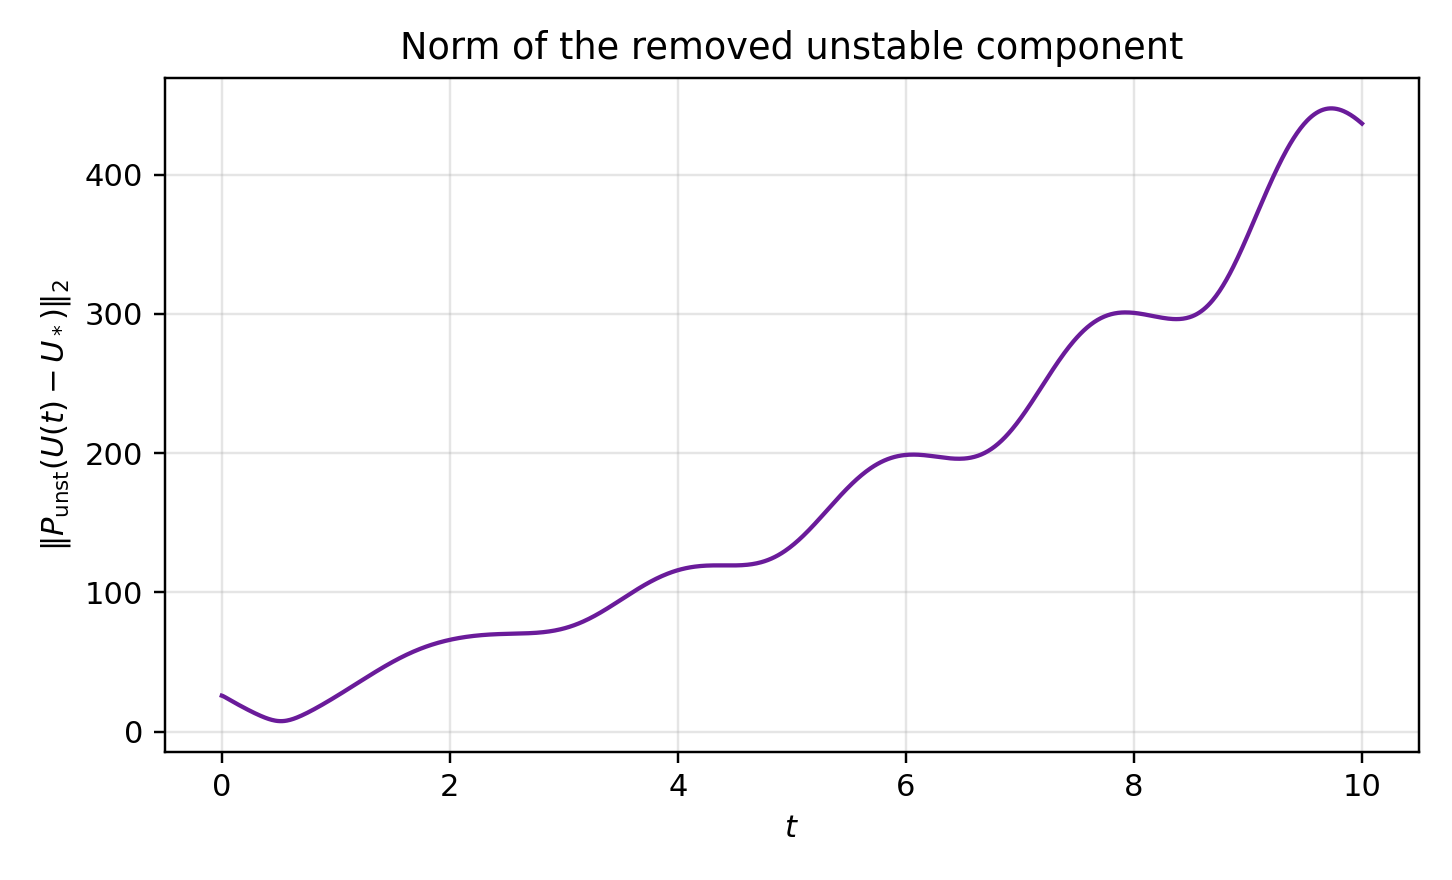
\includegraphics[width=0.82\textwidth]{images/projection_norm.png}
    \caption{Норма компоненты, вычтенной из исходных снимков при проекции на неустойчивое подпространство. Рост этой нормы показывает, что со временем траектория всё сильнее отклоняется от стационара именно вдоль неустойчивой моды.}
    \label{fig:projection-norm}
\end{figure}

На первом снимке норма проекции равна \(25.75\) после округления, а к последнему сохранённому снимку возрастает до \(436.69\).
Максимальное значение на рассматриваемом интервале составляет \(447.61\).
Это согласуется со спектральным анализом: положительная действительная часть \(\lambda\) приводит к накоплению амплитуды в неустойчивом направлении.

\begin{figure}[H]
    \centering
    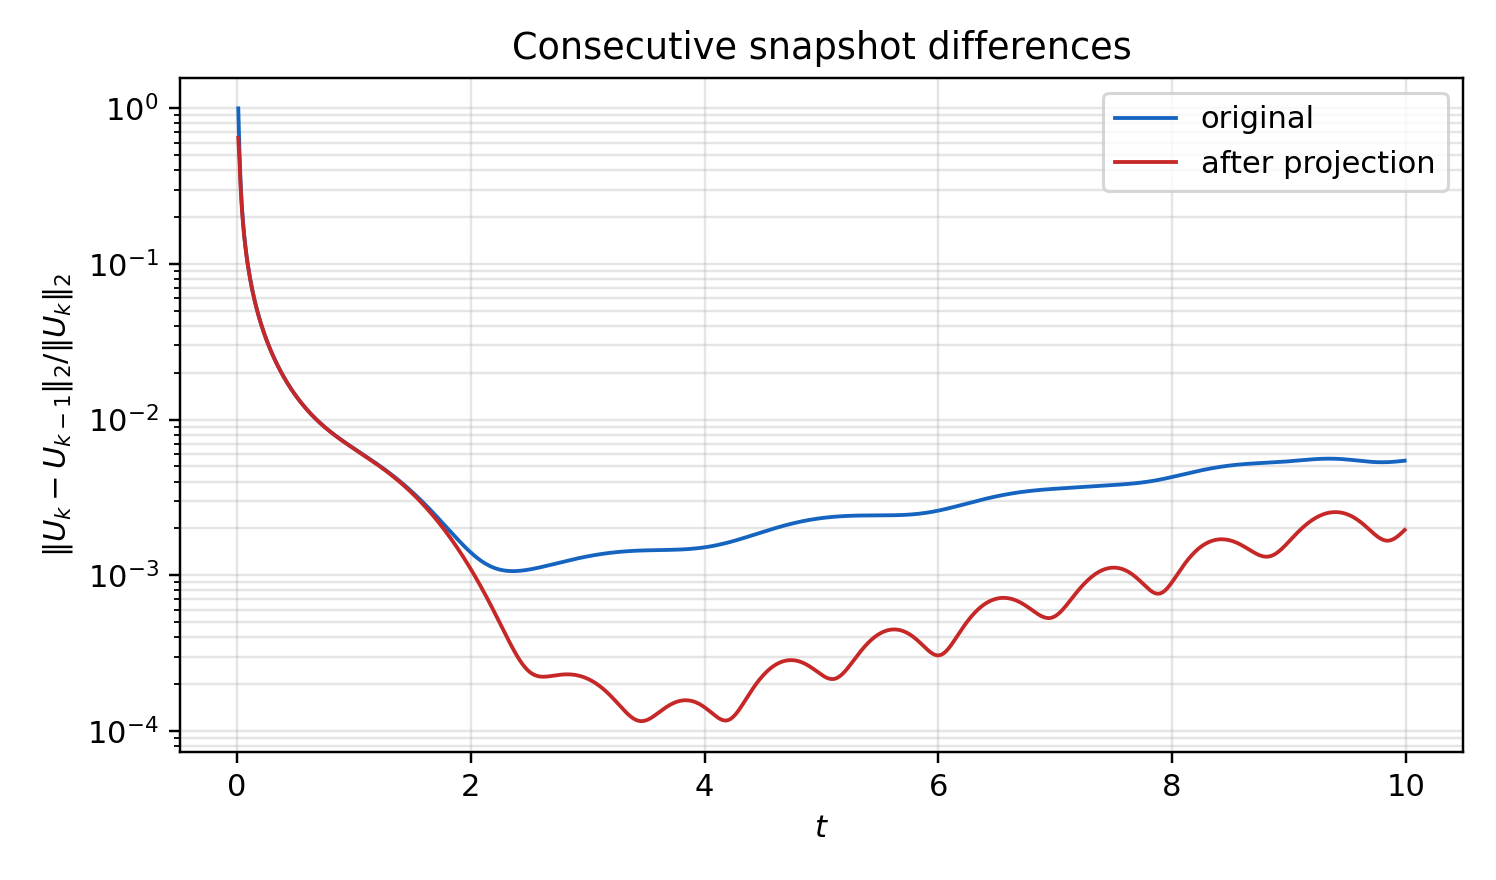
\includegraphics[width=0.82\textwidth]{images/raw_filtered_difference.png}
    \caption{Сравнение относительной разности соседних снимков до и после вычитания неустойчивых мод. После фильтрации минимум становится глубже, \(D_{\min}=1.15\cdot10^{-4}\) после округления, а поздний рост значительно слабее, чем в исходной последовательности.}
    \label{fig:raw-filtered-difference}
\end{figure}

До фильтрации минимальная относительная разность соседних снимков равна \(1.06\cdot10^{-3}\).
После вычитания неустойчивой компоненты минимум уменьшается почти на порядок:
\[
    D_{\min}^{\mathrm{filtered}}
    =
    1.15\cdot10^{-4}
    \quad \text{после округления, при } t=3.46001.
\]
На последнем сохранённом снимке исходная разность равна \(5.44\cdot10^{-3}\) после округления, а после фильтрации --- \(1.95\cdot10^{-3}\).
Это не означает, что решение стало строго стационарным.
Оно означает более тонкий факт: из решения удалена главная линейная неустойчивость, но остаются устойчивые колебательные компоненты, нелинейные эффекты и численная ошибка.

\begin{figure}[H]
    \centering
    \begin{subfigure}{0.49\textwidth}
        \centering
        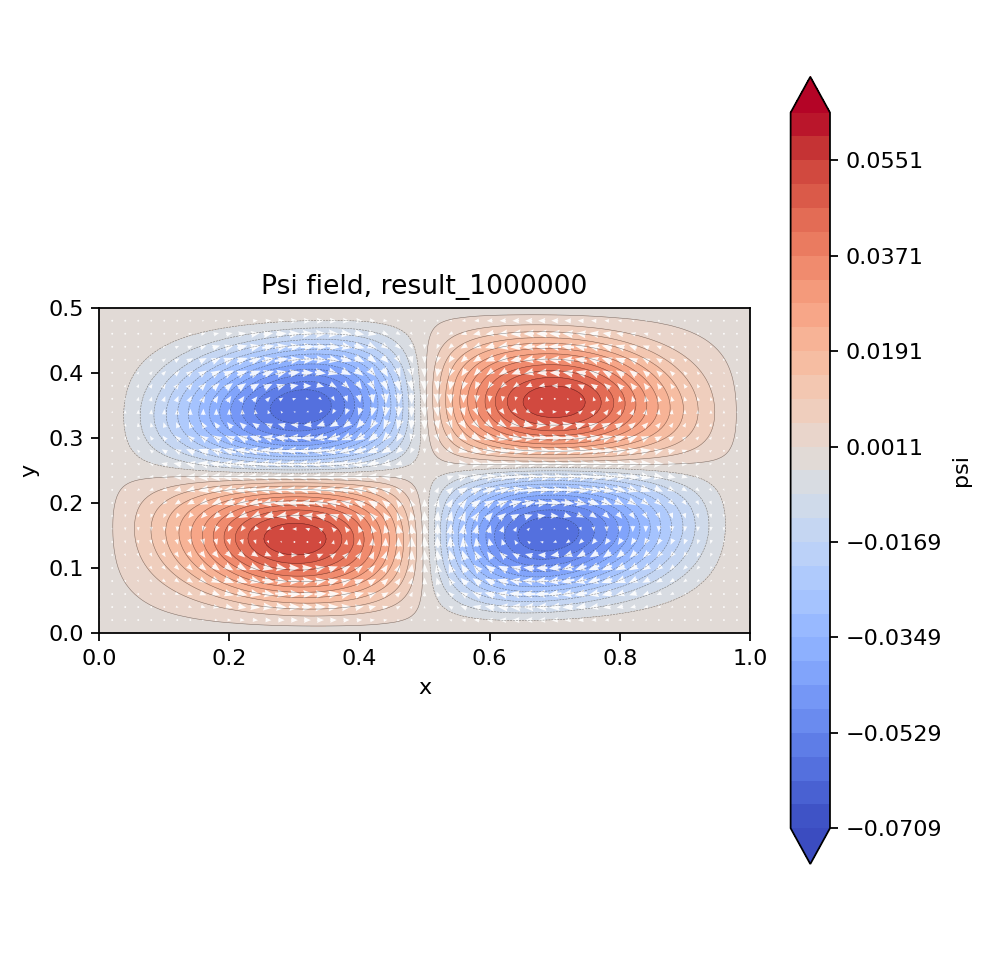
\includegraphics[width=\textwidth]{images/filtered_result_1000000_psi.png}
        \caption{\(\psi\)}
    \end{subfigure}
    \begin{subfigure}{0.49\textwidth}
        \centering
        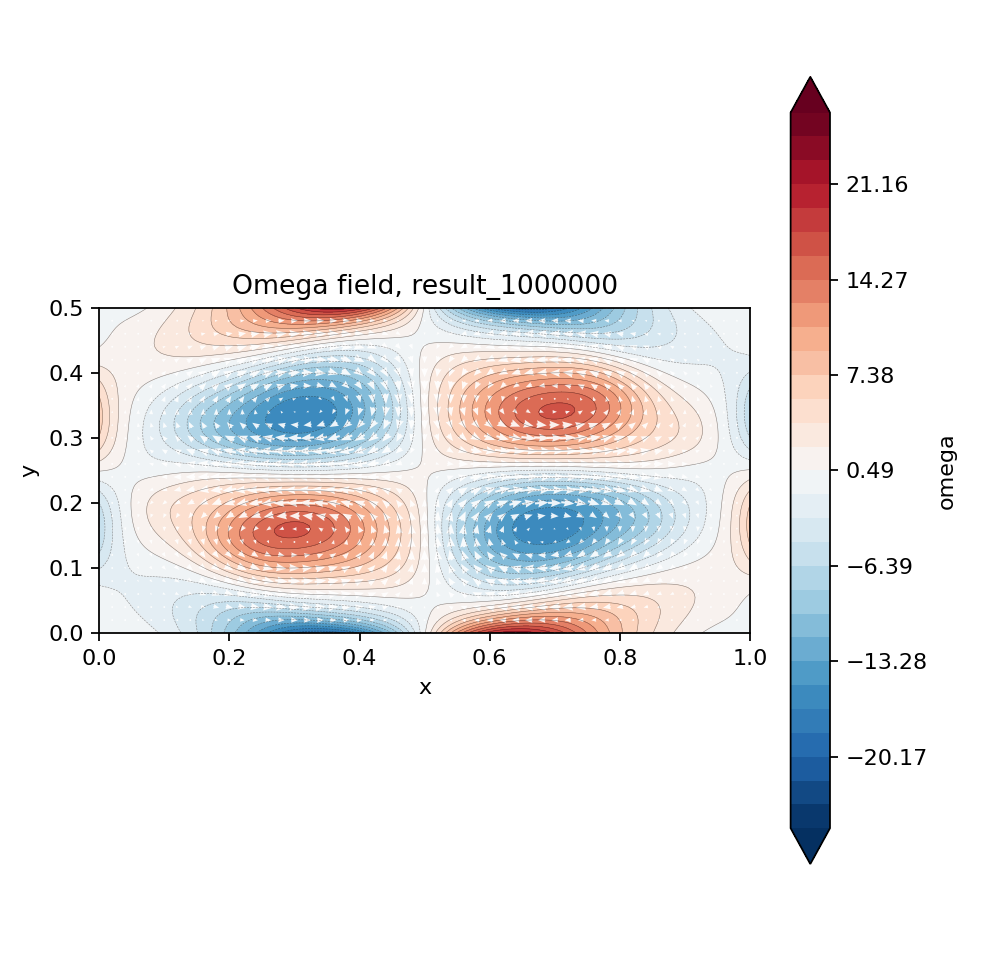
\includegraphics[width=\textwidth]{images/filtered_result_1000000_omega.png}
        \caption{\(\omega\)}
    \end{subfigure}
    \caption{Поля функции тока и завихренности после вычитания неустойчивых мод на шаге \(10^6\). По сравнению с \cref{fig:raw-fields} поле становится ближе к симметричному четырёхвихревому режиму, а амплитуда отклонения уменьшается.}
    \label{fig:filtered-fields}
\end{figure}

\begin{figure}[H]
    \centering
    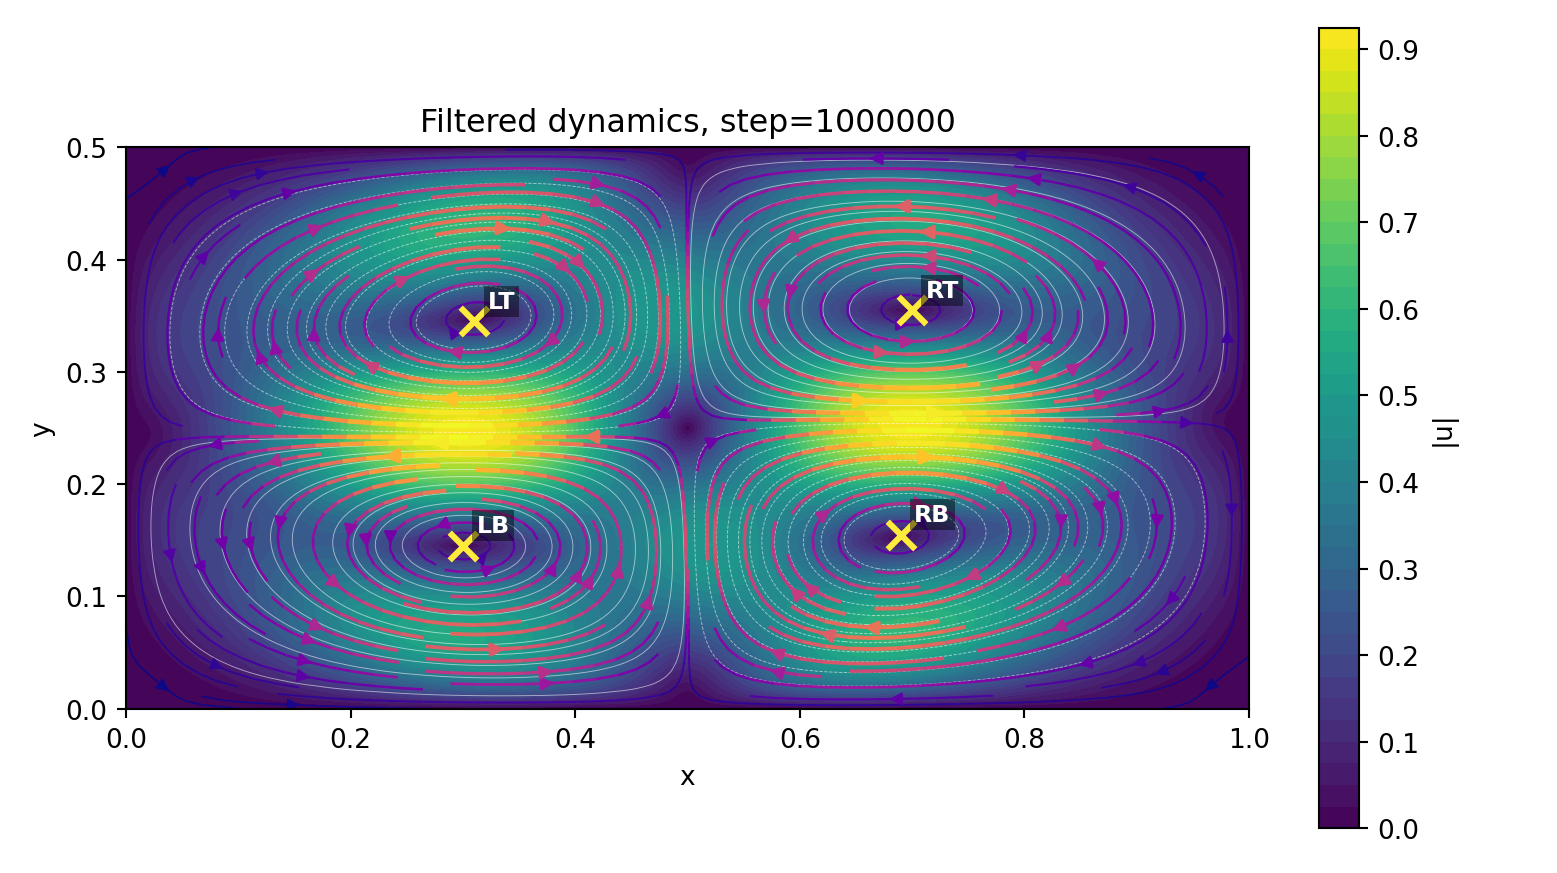
\includegraphics[width=0.88\textwidth]{images/pulsation_filtered_1000000_centers.png}
    \caption{Линии тока после фильтрации на шаге \(10^6\). Четырёхвихревая структура сохраняется заметно лучше, чем в исходном решении на \cref{fig:raw-streamplot}: центры вихрей возвращаются к расположению, близкому к кандидату на \cref{fig:stationary-candidate}. Это визуальное проявление удаления компоненты вдоль неустойчивого собственного направления.}
    \label{fig:filtered-streamplot}
\end{figure}

Количественно фильтрация уменьшает амплитуды полей.
Для исходного снимка на шаге \(10^6\)
\[
    \min\psi=-0.09835,\quad \max\psi=0.02764,\quad
    \min\omega=-20.94,\quad \max\omega=26.25.
\]
После фильтрации
\[
    \min\psi=-0.06143,\quad \max\psi=0.05427,\quad
    \min\omega=-19.85,\quad \max\omega=20.63.
\]
Скорости также становятся менее асимметричными:
\[
    |u|_{\max}=0.9208,\qquad |v|_{\max}=0.5001
    \quad \text{после округления}.
\]
Эти числа подтверждают визуальный вывод: фильтрация не уничтожает течение, а возвращает его ближе к четырёхвихревому стационарному режиму.

\section{Заключение}

В работе разобраны две связанные задачи вычислительной гидродинамики в переменных функция тока--завихренность.
Для задачи о каверне восстановлена математическая постановка непосредственно в переменных \(\psi,\omega\), включая граничное условие для функции тока и формулу Тома для завихренности.
Описана именно реализация с центральной аппроксимацией нелинейного члена: конвективный член аппроксимируется центральными разностями, а псевдовременная система решается факторизованным методом с прогонками по координатным направлениям.
Такая схема имеет второй порядок по пространству во внутренних узлах и первый порядок по псевдовремени.

Для форсированного течения в прямоугольной ячейке сформулирована модель сразу в переменных \(\psi\) и \(\omega\), как она используется в разностной реализации.
В текущей реализации используется равномерная сетка \(201\times101\), \(\Reynolds=1/\nu=260\), неподвижные стенки, внешняя синусоидальная форсировка и схема Аракавы для нелинейного члена.
Прямое интегрирование проходит близко к четырёхвихревому состоянию, но затем уходит от него, что видно как по графику разностей соседних снимков, так и по линиям тока.

Стационарное состояние было уточнено методом Ньютона--Крылова.
Далее система линеаризована около найденного стационара, и спектральный анализ выявил одну комплексно-сопряжённую неустойчивую пару собственных значений
\(\lambda=0.2170\pm1.7868i\) после округления.
Вычитание ортогональной проекции на вещественное подпространство, порождённое этой модой, заметно подавляет рост отклонения: минимальная относительная разность соседних фильтрованных снимков становится почти на порядок меньше, а поздняя динамика остаётся ближе к четырёхвихревой структуре.

Ограничения подхода также ясны.
Во-первых, фильтрация мод в этой реализации является численной процедурой постобработки, а не физически реализуемым граничным управлением.
Во-вторых, для раздела о каверне полезно провести полноценное сеточное исследование: текущие рисунки уже построены на сетке \(601\times601\), но для строгого вывода о сходимости нужно повторить расчёты на нескольких сетках и сравнить не только координаты центров, но и значения функции тока, завихренности и профили скоростей.
В-третьих, для метода Ньютона желательно сохранять историю невязки по итерациям, чтобы в отчёте была не только финальная картина стационара, но и полноценная диагностика сходимости.
Естественное дальнейшее развитие работы --- повторить расчёты на нескольких сетках, проверить сеточную сходимость, а затем заменить постобработочное вычитание мод на приближение к настоящему feedback-управлению, ближе к постановке~\cite{kornev2018}.

\begin{thebibliography}{9}

\bibitem{erturk2005}
Erturk E., Corke T.\,C., G\"ok\c{c}\"ol C.
Numerical solutions of 2-D steady incompressible driven cavity flow at high Reynolds numbers.
\emph{International Journal for Numerical Methods in Fluids}, 2005, Vol.~48, pp.~747--774.

\bibitem{kornev2018}
Kornev A.\,A.
Simulating the Stabilization Process by Boundary Conditions of a Quasi-Two-Dimensional Flow with a Four-Vortex Structure.
\emph{Mathematical Models and Computer Simulations}, 2018, Vol.~10, No.~3, pp.~363--372.

\end{thebibliography}

\end{document}
